% !Mode:: "TeX:UTF-8"
%\documentclass[10pt,draft]{IEEEtran}
\documentclass[10pt,conference]{IEEEtran}
\usepackage{subfig}
\usepackage{graphicx}
\usepackage{amsmath}
\usepackage{multirow}
\usepackage{algorithm}
\usepackage{algorithmic}
\usepackage{comment}
%\usepackage{ctex}

\graphicspath{figures/}

\newtheorem{theorem}{Theorem}
\newtheorem{lemma}{Lemma}
\newtheorem{definition}{Definition}

\begin{document}

\title{AVCS: Adaptive Virtual Channel Sharing Router Architecture for Networks-on-Chip}
%\onecolumn
%\author{\IEEEauthorblockN{Baoliang Li}}
\author{Baoliang~Li, %~\IEEEmembership{Student Member,~IEEE,}
        Zeljko Zilic, %~\IEEEmembership{Senior Member,~IEEE,}
        Wenhua~Dou, %~\IEEEmembership{Non-Member,~IEEE}% <-this % stops a space
\thanks{Baoliang~Li and Wenhua Dou are with the College of Computer Science, National University of Defense Technology, Changsha 410073, P.R. China}%
\thanks{Zeljko Zilic are with Department of Electrical \& Computer Engineering, McGill University, Montreal H3A-2A7, Quebec, Canada}%
\thanks{Manuscript received XX XX, 2014; revised XX XX, 2014.}}

\markboth{Journal of XXX,~Vol.~XX, No.~XX, XX~2014}%
{Li \MakeLowercase{\textit{et al.}}: Adaptive Virtual Channel Sharing Networks-on-Chip Architecture}

\maketitle

\begin{abstract}
The performance and hardware cost of wormhole-switched Networks-on-Chip (NoC) router heavily depend on the organization and management scheme of input buffer. In order to achieve high performance without introducing significant power and area burden, the management of buffer resources should adapt the dynamical change of traffic load. In this paper, we propose an inter-port Adaptive Virtual Channel (VC) Sharing router architecture, i.e. AVCS, which adjusts the VC number and buffer capacity each input port can use to improve the buffer utilization and network performance. Another contribution of this paper is that we introduce the idea of port sharing while implementing the VC Allocator (VCA) and SWitch Allocator (SWA), which utilizes a smaller VCA and SWA to meet the demand of large-scale VC and switch allocation. Based on a detailed RTL implementation, we evaluate the performance and hardware overhead of our proposal. Experimental results show that the proposed architecture saves 32.1\% power and 11.7\% chip area when compared with the typical router architecture with similar performance.
\begin{comment}
基于虚通道的虫孔交换片上网络的性能和成本严重的依赖于对片上缓存的组织和管理方式。为了最大化片上网络的性能并降低功耗和面积开销,片上缓存资源的分配和管理需要适应片上网络流量负载的动态变化并提高缓存的利用率。为此,本文提出了一种端口间缓存和虚通道共享的片上网络体系结构,该结构可以在运行时根据网络流量的变化动态的调整每个端口所能使用的缓存容量和虚通道数量,以提高网络性能和缓存利用率,达到以较少的硬件资源来实现较高的性能的目的。另外,为了降低虚通道和交换机分配器的规模,我们还提出了影子vc的概念,通过复用虚通道分配器和交换机仲裁器的端口来提高其端口利用率,在不影响性能的情况下实现以小规模分配器完成大量虚通道资源的分配的目的。基于一个详细的RTL硬件实现,我们评价了该方案的性能,并采用design compiler 基于45nm CMOS standard cell library 评估了该方案的硬件成本和功耗等指标。实验结果显示,与之前基于链表的动态缓存分配方案相比,我们的方案在热点流量下改进性能x\%,占用的芯片面积减少x\%。对于一个具体的VOPD应用,我们的方案较基于链表的方案性能提高\%x.与典型的虫孔交换的虚通道路由器相比,达到同样的的性能,我们的方案所需要的缓存资源减少x\%, 功耗降低x\%,面积减少x\%。
\end{comment}
\end{abstract}
\begin{IEEEkeywords}
Networks-on-Chip (NoC), VC sharing, buffer utilization
\end{IEEEkeywords}

\section{Introduction}
The wormhole-switched Networks-on-Chip (NoC) provides a scalable, high-performance and low-cost interconnection fabric for the large-scale Chip-MultiProcessor (CMP) and System-on-Chip (SoC). The performance, power and area of NoC router heavily depend on the buffer capacity and organization scheme. In a typical router \cite{DaTo01}, all the input ports have the same number of VCs and each VC is designated a fixed buffer capacity. Although the static structure eases hardware implementation, the buffer resources can not be fully utilized under some nonuniform traffic pattern. For the input ports with low traffic load, few buffer slots are enough to temporarily accommodate all the incoming flits that cannot be forwarded immediately, leaving the rest buffer resources of the same input port underutilized. In contrast, many buffer slots are necessary for the input ports with high traffic load to guarantee throughput. Since the buffer consumes more than 60\% power and chip area in a typical router \cite{1650108}\cite{ChPe03}, reserving large enough buffer space for each input port to ensure the performance under high traffic load is infeasible.
\begin{comment}
基于虚通道的虫孔交换片上网络为大规模片上多处理器系统和片上系统中核间通信提供了一种可扩展、高性能和低成本的实现方式。其性能、功耗和硬件成本都受到虚通道的数量、输入端口的缓存容量和缓存的组织方式的影响。传统的虚通道虫孔交换的片上网络路由器为每个端口分配相同数量的虚通道并为每个虚通道分配同样大小的缓存空间\cite{DaTo01}。这种静态分配的路由器结构虽然实现简单,但是在某些特定的流量模式下,其缓存资源得不到有效的利用。因为实际的traffic负载在片上网络中的分布通常是不均匀的而且是随时间动态变化的,traffic load较低的端口只需要较少的虚通道和缓存空间便可以保证吞吐率,而处于high traffic load的端口则需要较多的缓存空间和虚通道。类似的,同一端口内不同虚通道对缓存容量的需要也是不同的。为每个端口和每个虚通道分配较大的缓存容量虽然可以保证在高负载情况下的性能,但是会引入无法承受的芯片面积和消耗开销。因为有研究结果表明,片上网络60\%的功耗都是由缓存消耗的\cite{1650108}\cite{ChPe03}。
\end{comment}

The only way to implement a high-performance and low-cost NoC router is by improving the buffer utilization through appropriate buffer organization and management scheme. There have been significant works on this issue, e.g. \cite{NPKV06,4555894,6310960}. To improve buffer utilization, these approaches dynamically allocate buffer slots to each VC within an input port according to the traffic condition, which can achieve 50\% buffer saving without degenerating the network performance \cite{NPKV06}. In \cite{Neishaburi:2009:RAN:1531542.1531658}\cite{5770788},
inter-port buffer sharing scheme was proposed to further improve the performance and buffer utilization of typical router. Although all these approaches employ dynamical buffer management, the number of VCs each input port can use is fixed. We find that, these approaches can not fully exploit network performance with limited buffer resources under some scenarios. We take a $3\times 3$ mesh network employing Dimension Order Routing (DOR) as an example to illustrate one of these special cases, as shown in Fig. \ref{vcensuficent}. Packets from router 9 and 3 to router 5 are blocked due to lack of available VCs at North (N) and South (S) port of router 5. Whereas, 4 VCs in total at input port West (W), East (E) and Local (L) are idle. This example reveals that only sharing buffer resources among VCs and ports is not enough to maximize the performance of wormhole-switched NoC router, because the limited VC resources restrict the usage of buffer.
\begin{comment}
因此,并采用有效的缓存组织和管理方案来提高缓存利用率才是设计性能和成本均可接受的片上网络的解决办法。为此,研究者们提出了一类动态缓存分配的片上网络方案\cite{NPKV06}\cite{4555894}\cite{5770788}\cite{Neishaburi:2009:RAN:1531542.1531658}\cite{6310960}。 在这类体系结构中,路由器的每个端口仍然有相同数量的虚通道,但是每个虚通道所使用的缓存空间则是根据其对缓存的不同需求动态分配的。在相同的性能需要前提下,这类结构所需要的缓存容量仅为经典路由器结构的50\%。之后提出的端口间缓存共享方案\cite{Neishaburi:2009:RAN:1531542.1531658}\cite{5770788} 将动态缓存管理由端口内拓展到端口之间,进一步提升了路由器缓存资源的利用率。这类方案中,某个端口空闲的缓存可以被其它的端口使用,但是每个端口所能使用的虚通道的数量仍然是固定的。然而我们研究发现,在某些情况下,仅实现了端口内和端口间的缓存共享通常是无法最大化片上网络的性能的。图\ref{vcensuficent}以一个采用维序路由的3x3 mesh网络中的热点通信模式为例说明了这一点。节点9和3的报文由于路由器5的端口N 和S此刻没有足够的虚通道可用因而造成了阻塞,此时这两个端口的缓存也可不能得到有效的利用。而与此同时,路由器5 的W 和E 端口却有空闲的虚通道。
\end{comment}
\begin{figure}
  \centering
  \subfloat[All-to-1 Communication]{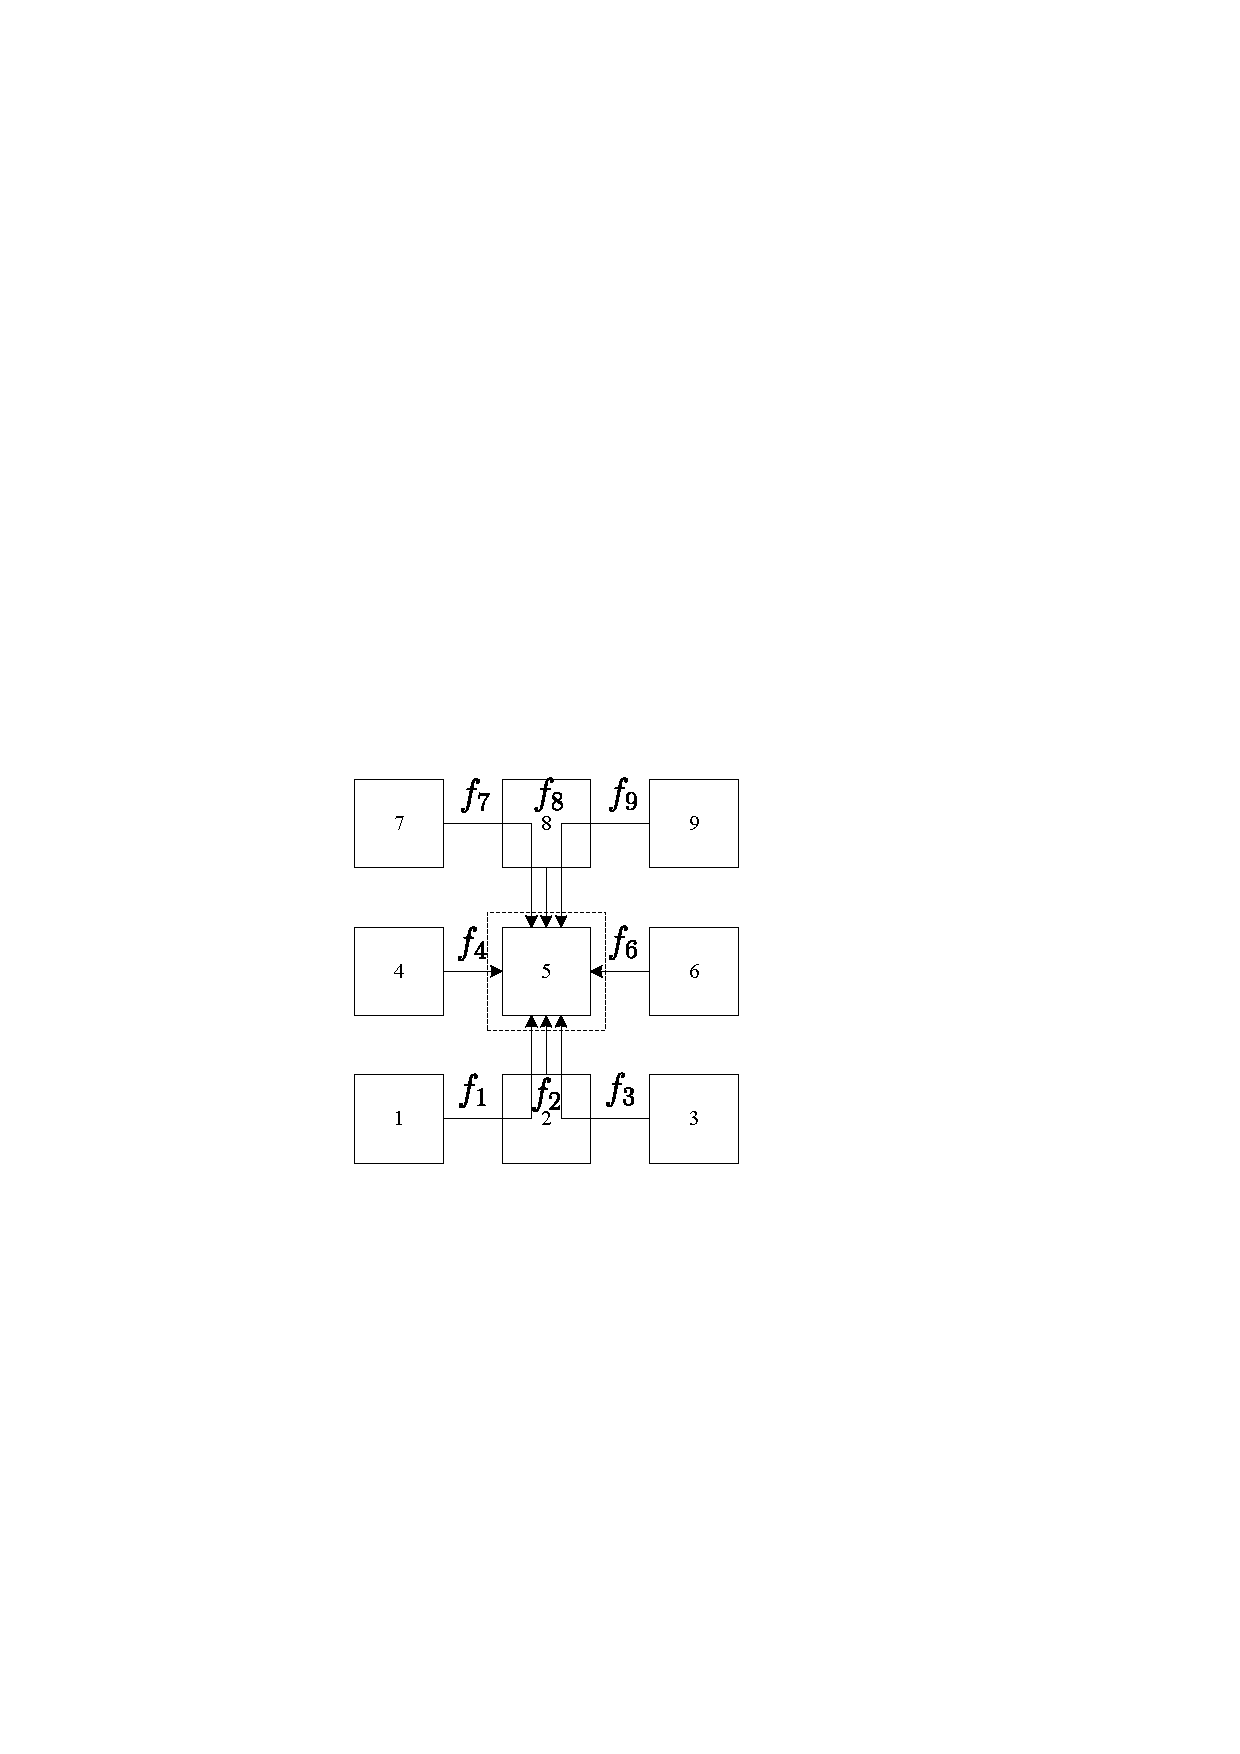
\includegraphics[scale=0.55]{figures/center.pdf}\label{center}}\hspace{10pt}
  \subfloat[VC Status of Router 5]{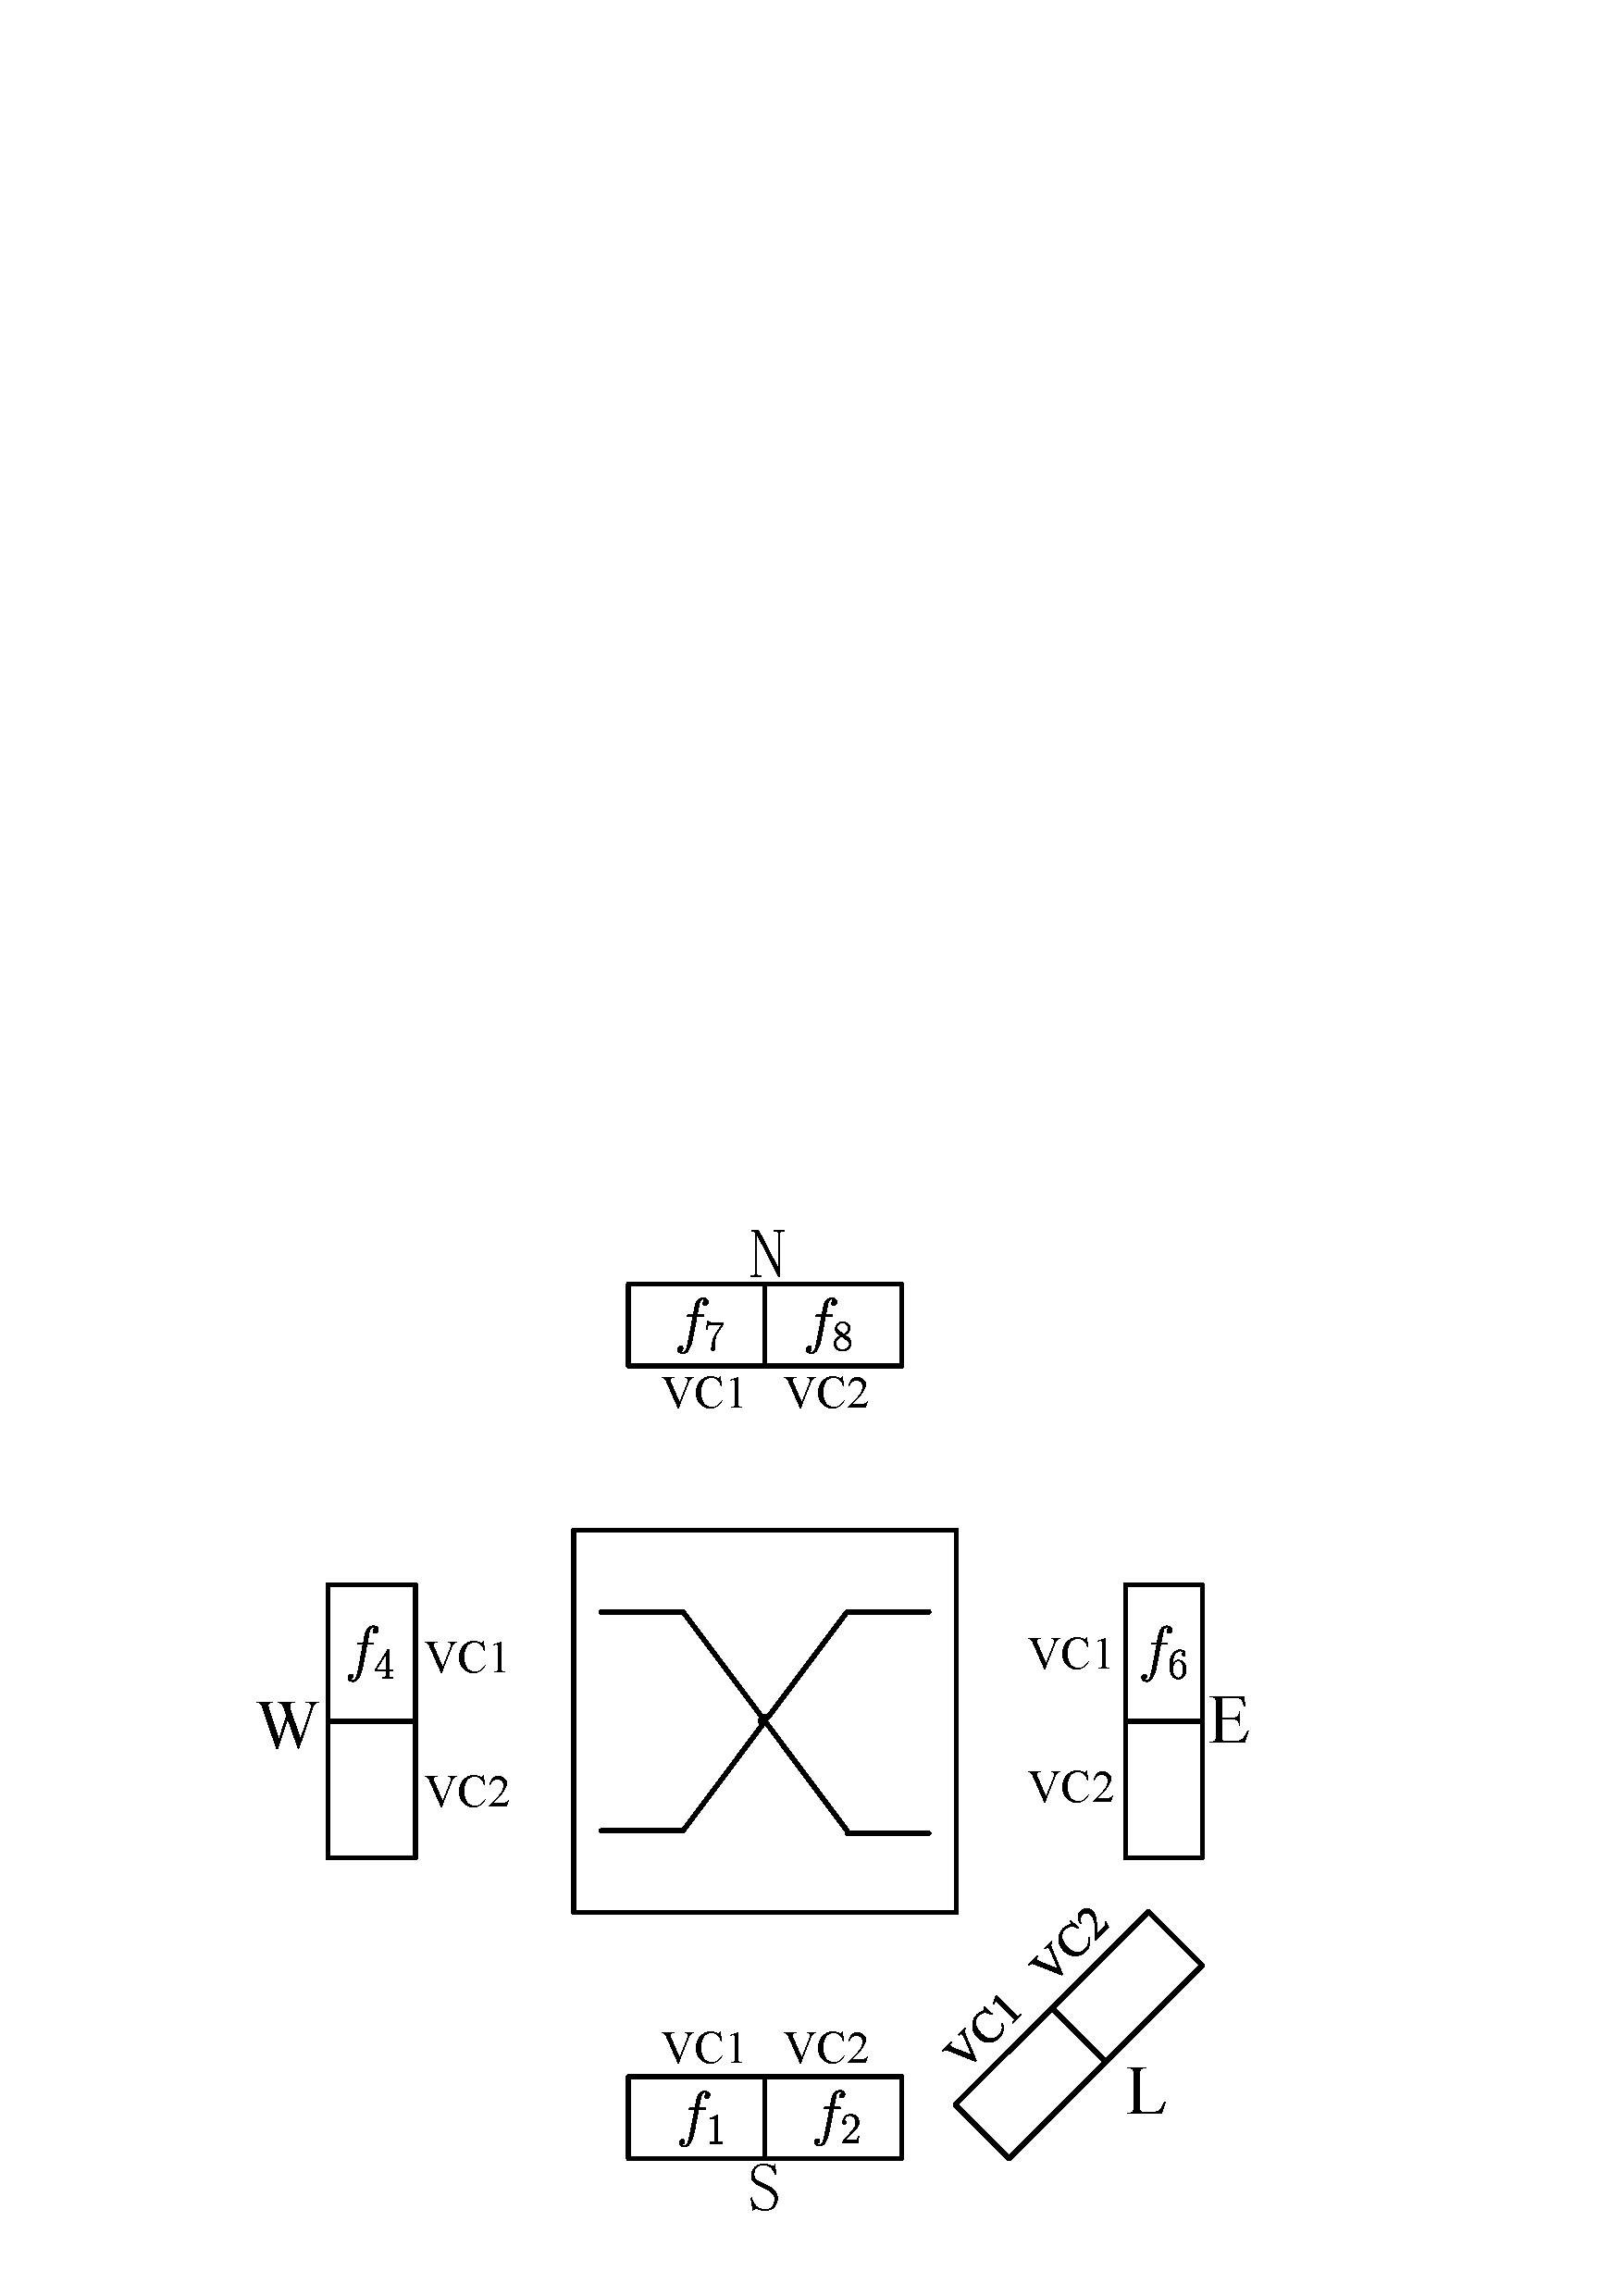
\includegraphics[scale=0.20]{figures/vcensufficient.pdf}\label{vcunbalance}}
  \caption{Blocking caused by VC insufficiency}\label{vcensuficent}
\end{figure}

Since the number of VC an input port required at any time instance is equal to the number of partial packets it accommodates, the VC resources required at each input port changes dynamically with time and traffic pattern. To avoid the blocking caused by VC insufficiency and guarantee the worst-case VCs requirement, an intuitive solution is that reserving large amount of VCs at each port. However, this solution is infeasible due to the follow two reasons: First, it introduces significant hardware overhead to manage and keep the status of each VC. Second, it makes the VC Allocator (VCA) and SWitch Allocator (SWA) very complex and further limits the frequency of router, because these two components usually lay on the critical path of entire router pipeline. We also noticed that, the average port utilization of VCA and SWA in typical router is very low. For an $N\times N$ mesh network, supposing each router has $P$ input and output ports, and each output port has $V$ VCs. Then, an VCA matches $P\times V$ request to $P\times V$ VCs. We define the average utilization of VCA as
$$\rho=\frac{1}{N^2PV}\times \sum_{n=1}^{N^2}\sum_{p=1}^P\sum_{v=1}^V\frac{ActiveCycles_{n,p,v}}{SampleCycles}$$
where $SampleCycles$ is the duration of sample period and $ActiveCycles_{n,p,v}$ is the number of cycles that the $v$th VC at $p$th input port of router $n$ request for an output VC. For the many-to-1 communication scheme shown in Fig. \ref{vcensuficent}, supposing each input port of a router is deployed with 16 buffer slots and 2 VCs. We change the packet length $L$ from 2 to 16 flits, and collect the average utilization of VCA under different injection rate. As indicated in Fig. \ref{utilization}, for the same injection rate, the average utilization decreases significantly while increasing the packet length. Because only the head flit of a packet can issue VC allocation request. Even near the saturation point of each configuration, the average utilization of VCA is less than 10\%. This observation motivates us to design new VC and switch allocator to improve the utilization and meet the same arbitration demands with lower hardware cost.
\begin{figure}
\centering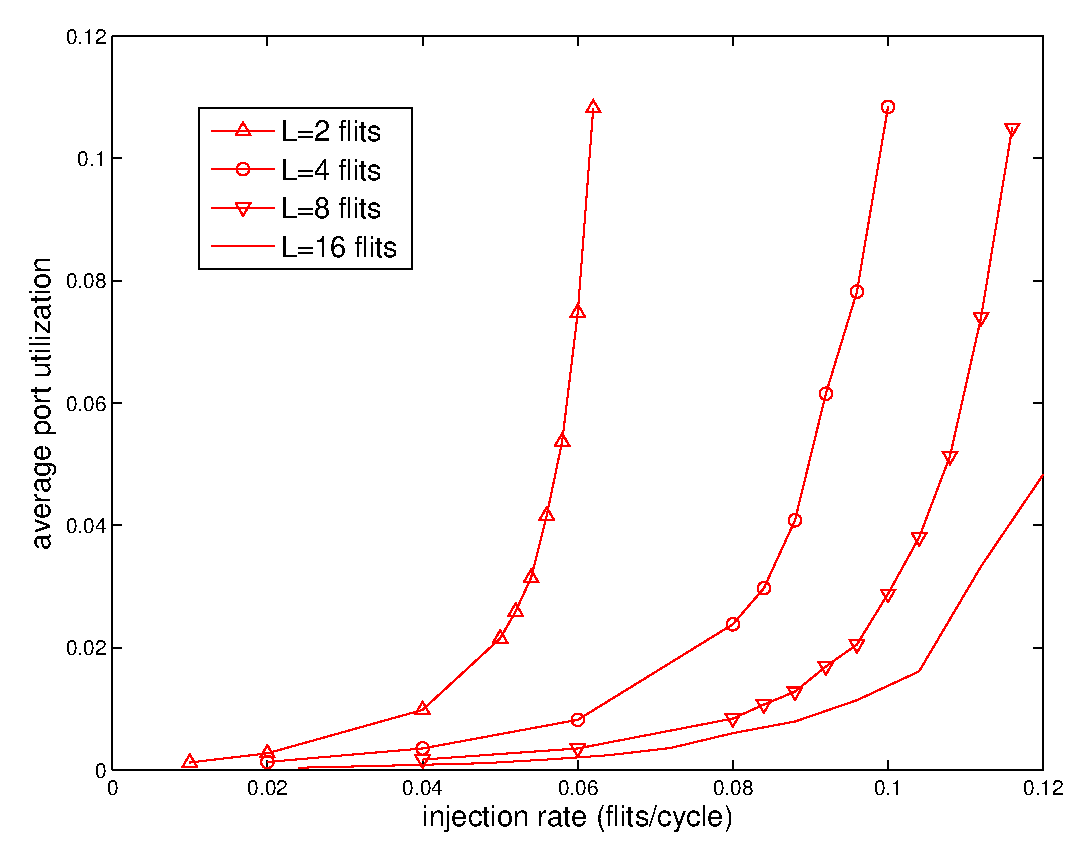
\includegraphics[scale=0.5]{figures/util.eps}
\caption{The port utilization of VC allocator under different injection rate and packet length.}\label{utilization}
\end{figure}
\begin{comment}
为了减少或者避免因虚通道不足引起的阻塞,一个直接的办法是为每个端口预留大量的虚通道以保证在路由器在最差情况下的性能。但是存在以下两个问题:一方面维护大量的虚通道状态会引入了较大的硬件开销,另一方面虚通道分配器和交换机分配器复杂度的提高也会进一步限制片上网络所支持的最高频率。由于某个网络端口在某个时刻所需要的虚通道的数量等于该端口当前所要容纳的不完全报文的数量,因此片上网络中不同的端口所需要的虚通道数量是随机流量模式和时间动态变化的\cite{1420211}。
\end{comment}

In this paper, we propose an inter-port Adaptive VC Sharing (AVCS) router architecture, which improves network performance and alleviates the blocking caused by both flow control and VC insufficiency by sharing VC and buffer resources among different input ports. Our approach reserves some VC resources for each input port and leaves the other VCs shared by all the input ports. Under low traffic load, the private buffer and VCs are enough to hold all the incoming packets. While under high traffic load, the shared VCs and buffer can be employed to alleviate the blocking caused by both flow control and VC insufficiency. Another contribution of this paper is that we propose the idea of request port sharing to reduce the complexity of VCA and SWA, which multiplexes the request ports of VCA and SWA between shared VCs and private VCs. This scheme allows us to employ small-scale VCA and SWA to arbitrate among large amount of VC request.
\begin{comment}
为此,我们提出一种结合的端口间缓存和虚通道共享的片上网络体系结构,通过降低每个端口的报文因流量控制和vc分配失败造成的阻塞和停顿来改进平均网络延迟并提升吞吐率。我们的方案为每个端口分配一定数量的私有VC和缓存容量,并在端口之间共享一定数量的动态VC和缓存。 当某个端口的负责较轻时,私有VC和缓存足够支持切片数据的无阻塞移动。而当某些端口的负载较重时,共享的buffer和虚通道则可以用来缓存大量的切片。另外,为了降低虚通道分配器和交换机分配器的复杂度,我们提出了影子vc的概念,使得可以用较小规模的仲裁器来实现对大量vc的仲裁,从而使得vc和sw 仲裁器的利用率和最高工作频率成为可能。与之前vichar\cite{NPKV06}等动态缓存管理方案不同的是,我们的方案基于传统的路由器结构进行修改得到,不需要对整个路由器结构进行重新设计和实现。而且新增加的共享缓存分配模块与路由器流水线并行的独立的操作,不会对路由器的关键路径产生不利的影响。
\end{comment}

The reset of this paper is organized as follows: A summary of related work follows in Section \ref{related}. We introduce the micro-architecture of AVCS in Section \ref{implemented}. Related experimental results are presented in Section \ref{experiemnts}. Finally, we conclude this paper and give the future work in Section \ref{conc}.
\begin{comment}
本文余下章节的安排如下:第\ref{related}节介绍相关的研究现状,第\ref{implemented}节介绍我们提出的路由器体系结构,相关的实验结果在第
\ref{experiemnts}节给出。最后,我们在第\ref{conc}节对本文进行总结并指出futher work。
\end{comment}

\section{Related Work}\label{related}
The input buffer accounts for a large fraction of the overall area and power budget of typical NoC router \cite{1650108}\cite{ChPe03}. Thus, reducing buffer capacity and improving buffer utilization is essential to implement a high-performance NoC router without introducing significant hardware overhead. A proper buffer organization and management scheme is necessary to increase the buffer utilization of wormhole-switched NoC router. There have been significant works focusing on this issue, and several solutions have been proposed.
\begin{comment}
有研究表明,input buffers account for a large fraction of the overall area and power budget of typical Network-on-Chip\cite{1650108}\cite{ChPe03},而且存储一个报文消耗的能量要多于在链路上传输所消耗的能量\cite{1012681}。因此,减少缓存容量并提高缓存利用率是在保证性能的前提下降低片上网络功耗和实现开销的唯一办法。Proper buffer sizing and organization are essential to increase buffer utilization. 为了解决静态的缓存分配方法缓存利用率低的问题,一些虚通道动态缓存分配的体系结构已经被提出。
\end{comment}

Virtual Channel Regulator (ViChaR) proposed in \cite{NPKV06} utilizes a table-based Unified Buffer Structure (UBS) to dynamically allocate the buffer slots for each VC according to the traffic condition. Although the buffer utilization and network performance are greatly improved, it introduces significant power burden due to the introduction of additional control logic. The router architecture based on Dynamically Allocated Multiple Queue (DAMQ) \cite{liu2006shared} can provide better performance than typical router while keeping the hardware cost low. To eliminate the additional three-cycle delay of conventional DAMQ structure, a prefetch mechanism was proposed in \cite{6310960}. In \cite{4555894}, the authors proposed a Linked-List based buffer Structure (LLS) and congestion avoidance scheme to improve the network performance and reduce the power and area cost of NoC router. An VC renaming mechanism was proposed in \cite{6296442} to virtualize the physical VC and increase the robustness of NoC router in case of failure. In addition, to alleviate the performance degradation caused by coupling among VCs, an adaptive back-pressure mechanism was proposed in \cite{BeckerJMD12}.

In \cite{Neishaburi:2009:RAN:1531542.1531658}\cite{5770788}, inter-port buffer sharing was proposed to further improve the buffer utilization of typical router. The control logic of this fully shared scheme is more complex than the intro-port buffer sharing schemes, which introduces significant hardware overhead \cite{Park2008}. Accordingly, a similar inter-port buffer-stealing scheme for the normal router without VC was proposed in \cite{5722177}. To alleviate the addition control overhead of fine-grained buffer sharing, a Partial Virtual Channel Sharing NoC (PVS-NoC) was proposed in \cite{5739053}, which shares some FIFO buffer between neighbor input port.
\begin{comment}
Virtual Channel Regulator (ViChaR) was proposed in \cite{NPKV06}, which utilize a table based unified buffer structure (UBS) to dynamically allocate the buffer resource for each virtual channel according to the traffic condition. 尽管提高了一个端口内部的buffer 利用率\cite{Park2008},ViChaR也提高了设计的复杂性和功耗。A novel Dynamically Allocated Multiple Queue (DAMQ) was proposed for NoC systems \cite{liu2006shared}, which provides the same performance while keep the hardware cost very low. To eliminate the additional three-cycle delay of conventional DAMQ, a prefetch mechanism for DAMQ is proposed in \cite{6310960}. In \cite{4555894}, the authors proposed an linked list based buffer structure and a congestion avoidance scheme to improve the network performance and reduce the power and area cost of NoC.前面提到的方法只解决了端口内的缓存区动态分配问题, in \cite{Neishaburi:2009:RAN:1531542.1531658}\cite{5770788}, Inter-port buffer sharing was proposed to further improve the buffer utilization of entire router. 其中,MH提出的RAVC方法虽然支持动态VC容量以避免HoL,但是控制罗男过于复杂,硬件成本过高,需要大量的额外的存储器和寄存器文件来存储控制信息,而且RAVA的方法基于Vichar的方法,只能用于固定报文长度。Accordingly, An similar inter-port buffer-stealing scheme for the normal router without VC was proposed in \cite{5722177}. To avoid addition control cost of fine-grained buffer sharing, a Partial Virtual Channel Sharing NoC (PVS-NoC) is proposed in \cite{5739053}. 该方法假设某些路由端口之前有一部分FIFO是可以被两个端口共享的;An Virtual Channel Renaming mechanism is proposed in \cite{6296442} for NoC to virtualize the physical VC and increase the robustness of NoC in case of failure.另外,为了避免一个病态的数据流占用较多的缓存空间而引起的性能下降,an adaptive backpressure机制在\cite{BeckerJMD12}中提出。对于端口间的动态缓存管理,还有一类粗粒度的共享方法,该类方法采用较多的分布式buffer来模拟输出缓存的交换结构\cite{Soteriou:2009:HDS:1591872.1591936}以提高吞吐率,但是其缓存利用率和功耗效率很低。
\end{comment}

The common characteristic of all these proposals is that they reserve large amount of VCs at each port and share buffer resources among VCs to improve buffer utilization and network performance. Whereas, reserving too many VCs introduces significant hardware overhead and makes the utilization of VCA and SWA very low. In addition, under some real-world traffic pattern, the uniformly distributed VC architecture is inefficient because it can not adapt the dynamical change of network traffic. Thus, only combining the buffer sharing and VC sharing can we implement a high-performance NoC router without introducing significant hardware overhead.
\begin{comment}
所有这类动态VC分配方案的本质是为每个端口分配大量的VC,并实现同一个端口内的不同VC的动态缓存分配. 由于虚通道的规模可以保证在最差情况下的性能,在实现运行过程中虚通道和交换机分配器的端口的利用率是非常低的。另外,在X-Y路由条件下,X方向更加容易拥塞\cite{KiNP06},这种不均衡也导致之前的均匀和静态vc分布方案存在很大的问题。因此,只有同时结合了端口间动态缓存和虚通道共享,才可以使用有限的硬件资源同时降低流量控制阻塞,交换机分配阻塞和虚通道分配阻塞。本文中我们便实现了这样一种方式。
\end{comment}

\section{Proposed AVCS Router Architecture}\label{implemented}
\subsection{Key Design Consideration}
Virtual channel provides a way to multiplex the physical channel in wormhole-switched NoC to reduce the Head-of-Line (HoL) blocking and deadlock. To avoid packet interleaving, an VC can only be reallocated when the tail flit of previous packet has been completely transmitted to the downstream router. If all the VCs have been occupied, blocking occurs because the packets from upstream router can not find an available VC at downstream router. The degradation caused by VC insufficiency is much serious than that of flow control, especially when the packet size is very large. One solution to this problem is that reserving large amount of VCs for each input port, e.g. \cite{NPKV06}\cite{4555894}\cite{5770788}\cite{Neishaburi:2009:RAN:1531542.1531658}\cite{6310960}. Whereas, it makes the VCA and SWA very complex, and a large amount of registers should be used to track the state of VC resources. Another promising approach is by sharing the buffer and VCs among all the input ports, and allocate buffer and VC resources on demand according to the traffic condition and the VC status of each input port.

While designing the inter-port buffer and VC sharing scheme, the following four issues should be considered:
\begin{comment}
vc是维持报文内部切片以正确的顺序传输的有效手段。为了防止报文交叠,只有当某个报文的尾切片已经被正在输出以后该虚通道才能被分配给新的报文使用。如果因为某些原因,已经分配了vc的报文因某些原因被阻塞而无法前进,那么此时没有分配到vc的报文在即使前方没有阻塞也无法传输。因此,因虚通道不足引起的阻塞对网络性能的影响远远大于因流量控制引起的拥塞,特别是当报文长度很长时。解决需通道阻塞的一个办法是为每个端口预留大量的虚通道,例如\cite{NPKV06}\cite{4555894}\cite{5770788}\cite{Neishaburi:2009:RAN:1531542.1531658}\cite{6310960}。 但是这会使得虚通道分配和交换机仲裁变得十分复杂。另外,为每个端口预留大量的虚通道也会消耗大量的寄存器资源来跟踪与该vc相关的报文的情况及传输状态等。另一种promising的方法是,在路由器端口之间实现虚通道和缓存共享,在运行过程中根据每个端口的流量和虚通道使用情况来动态的为每个端口分配虚通道和缓存。但是,在设计端口间缓存共享的方案时还有以下几个问题需要考虑:
\end{comment}
\begin{enumerate}
\item Interference caused by buffer sharing: When buffer resources are shared among input ports, an adversarial workload injected from one input port might monopolize all the buffer space of the other input ports and cause global congestion. Thus, special care should be taken to prevent the blockage from spreading to other ports.
\begin{comment}
(1)因端口间缓存共享带来的interference问题。在\cite{BeckerJMD12}中作者揭示了端口内动态缓存管理方案中因为个别虚通道占用所有缓存空间使得其它数据流产生流量控制阻塞而造成的性能下降现象。类似的现象在完全端口间缓存共享时也会出现,考虑某个端口将其它端口的缓存区全部占用时带来的性能下降。
\end{comment}
\item Read/Write conflicts caused by buffer sharing: Since each buffer bank can be accessed by multiple input ports, potential conflicts might occur when multiple input ports trying to access the same bank. Thus, additional read/write control logic and scheduling policies should be implemented to avoid hazard.
\begin{comment}
(2)共享存储体的读写冲突问题。在实现端口间缓存共享时,需要认真考虑因几个端口同时对同一个共享存储体进行读写时可能出现的冲突。
\end{comment}
\item Trade-off between hardware overhead and performance: Although the inter-port buffer sharing can further improve the performance of typical router, it introduces additional hardware overhead. Thus, the trade-off between performance and hardware overhead is necessary to design a high-performance NoC router with acceptable hardware overhead.
\begin{comment}
(3)端口间缓存共享的硬件成本和潜在的性能优势。完全缓存共享可以最大限度的利用路由器的缓存资源以减少因流量控制造成性能下降,但是会引入巨大的硬件开销。在设计时需要在成本和性能之间进行折中。
\end{comment}
\item The complexity of VCA and SWA: When inter-port VC sharing is implemented, the maximal number of VC each input port can use is equal to the total number of private VCs and shared VCs, which is larger than that of typical router. Thus, special care should be taken while designing VCA and SWA, since they occupy large chip area and restrict the frequency of router.
\begin{comment}
(4)虚通道和交换分配器的规模问题。对于每个路由器端口来说,它能使用的最大的虚通道数量$V_{max}$等于私有虚通道的数量加上共享虚通道的数量,远远大于没有实现共享的方案。规模庞大的虚通道和交换机分配器会占用大量的芯片面积并影响路由器所能支持的最高频率。
\end{comment}
\end{enumerate}

\subsection{Proposed Micro-architecture}
Taking all these aspects into consideration, we proposed the Adaptive VC Sharing (AVCS) NoC router architecture, as shown in Fig. \ref{architecture}. This proposal realizes partial buffer and VC sharing: each input port contributes a small portion of their buffer and VC resources to form shared buffer banks. All these shared buffer banks have an unique bank ID, which can be accessed by all the input ports of a router. For an AVCS router with five input ports, there are five banks in total, and each shared bank manages their own buffer space independently. The owner of each shared buffer bank is determined by their own shared buffer allocator ($\textcircled{4}$ in Fig. \ref{architecture}). The buffer allocator is a Finite State Machine (FSM), which grants a new owner according to the traffic condition of each input port whenever this bank keeps idle for several cycles.
\begin{figure*}
  \centering
  \subfloat[Proposed AVCS router micro-architecture.]{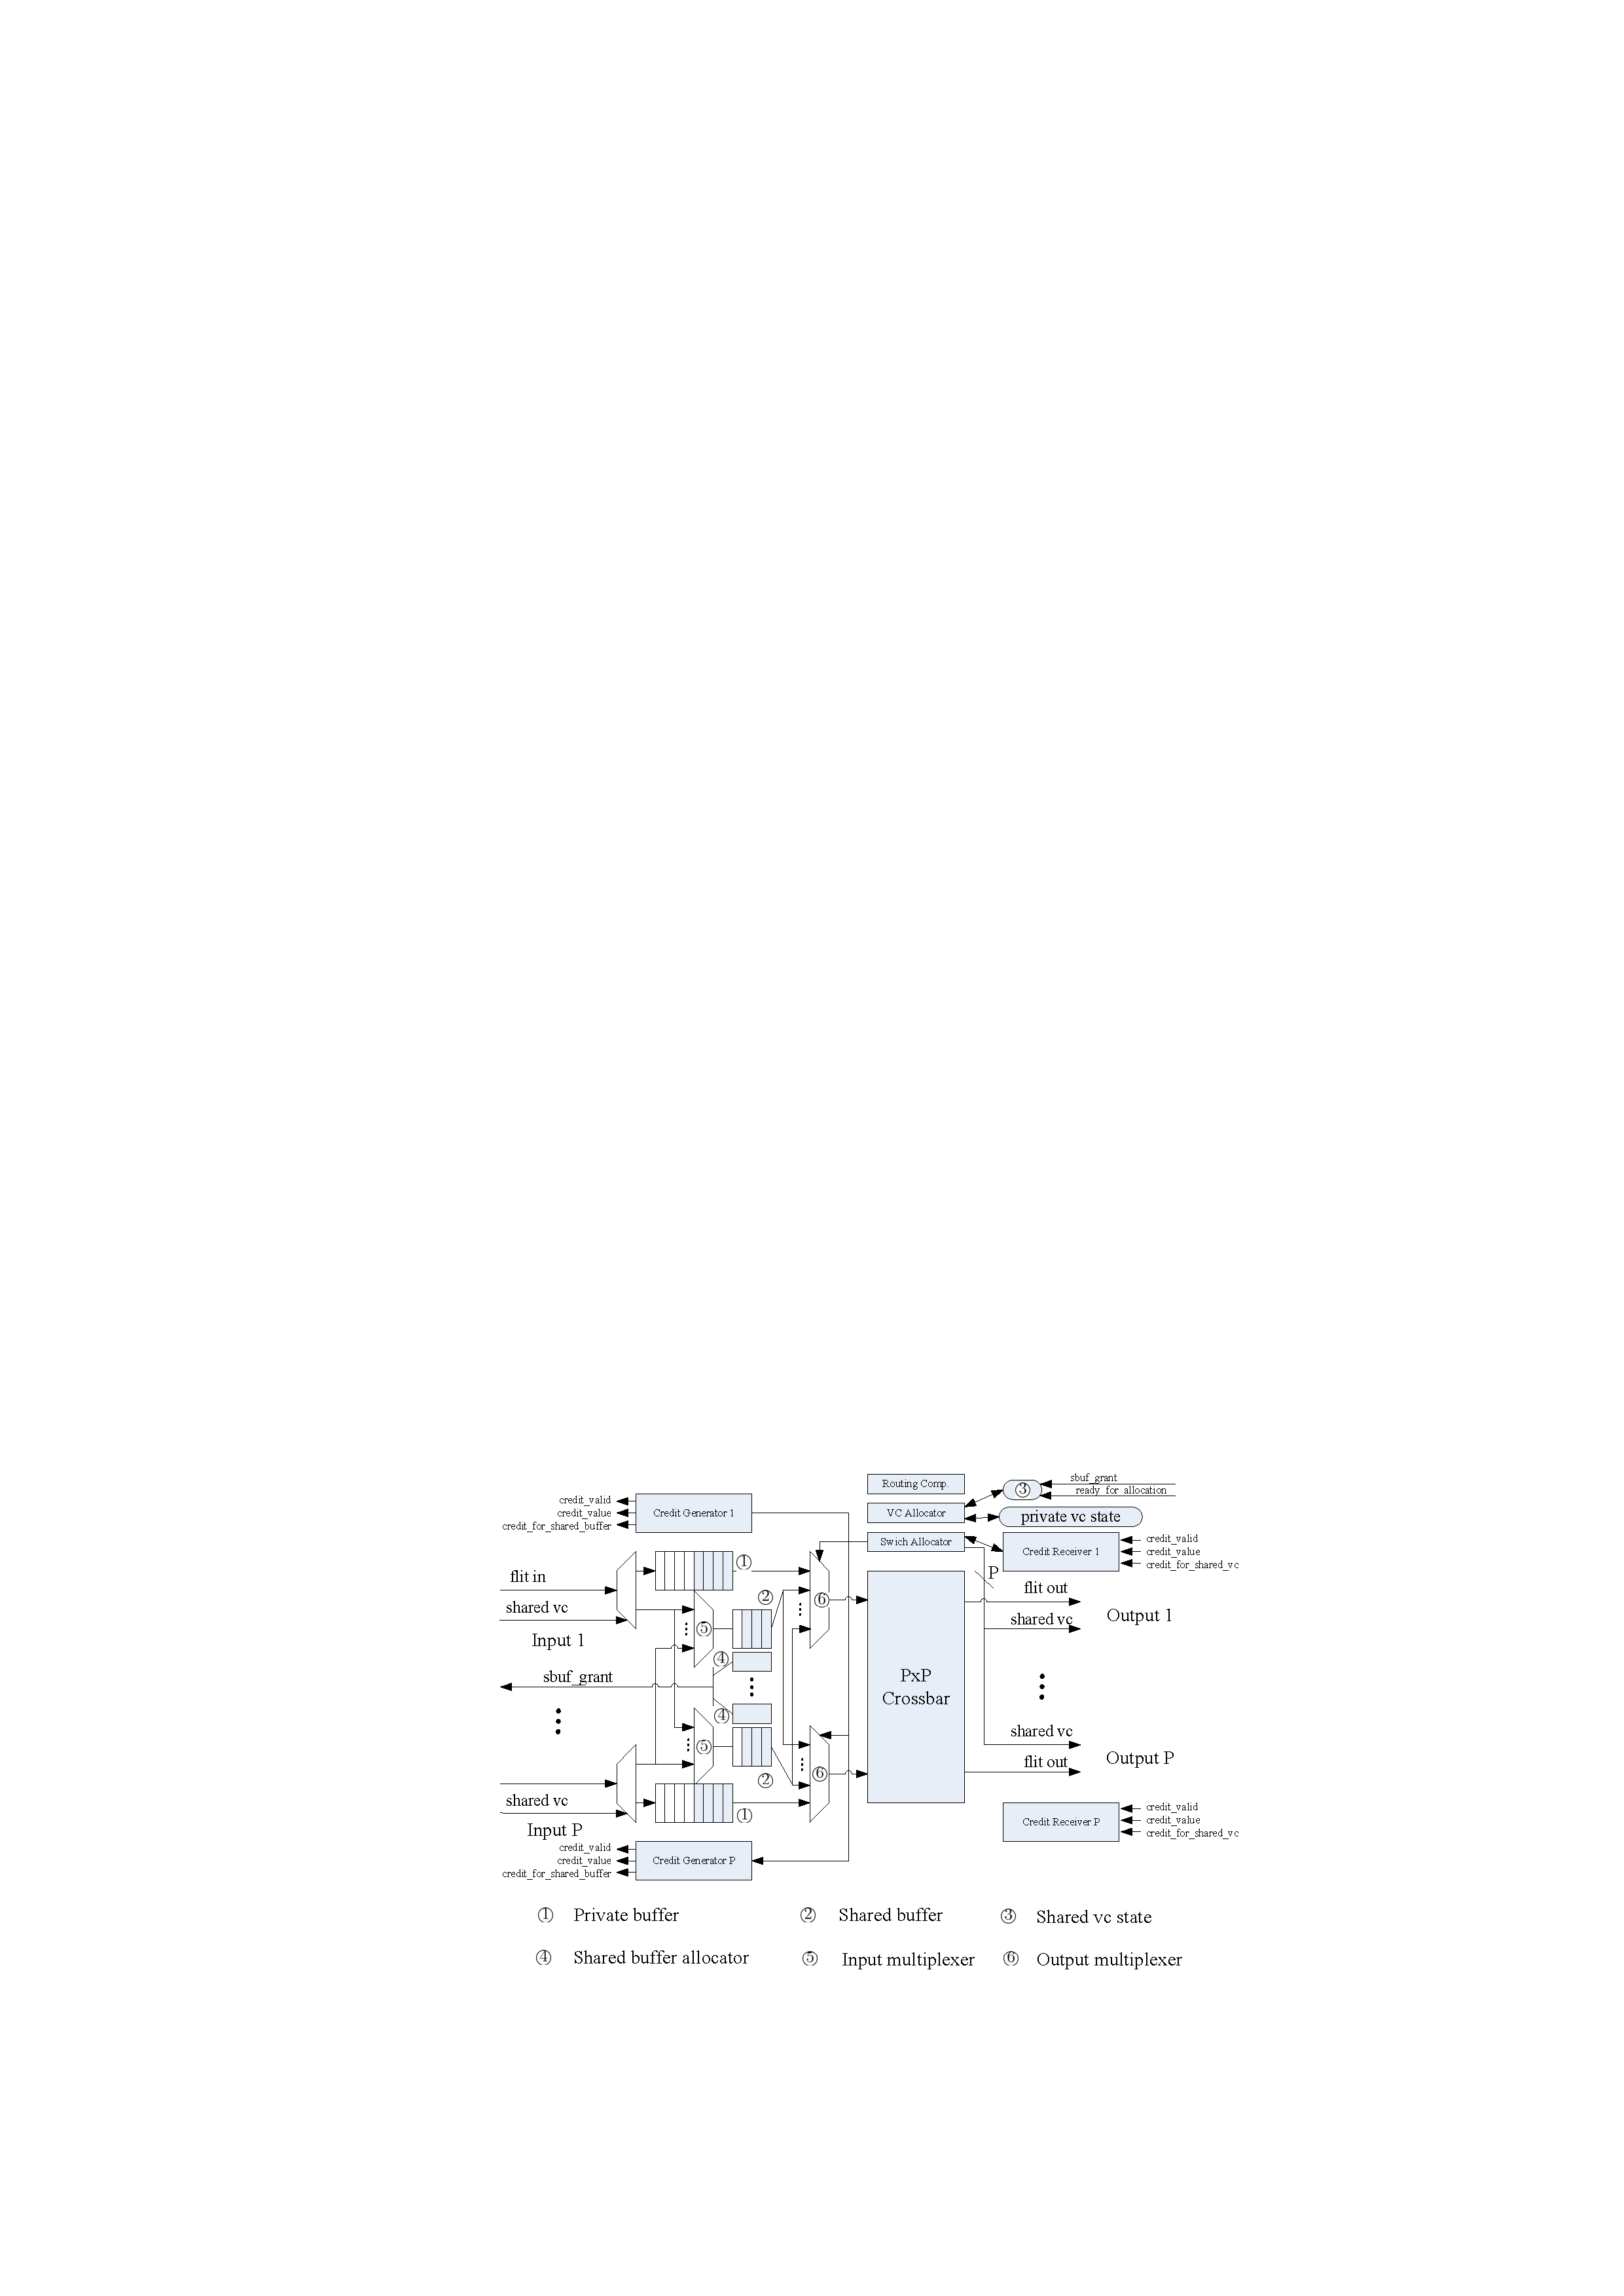
\includegraphics[scale=0.45]{figures/architecture.pdf}\label{architecture}}\hspace{10pt}
  \subfloat[The internal structure of shared/private buffer]{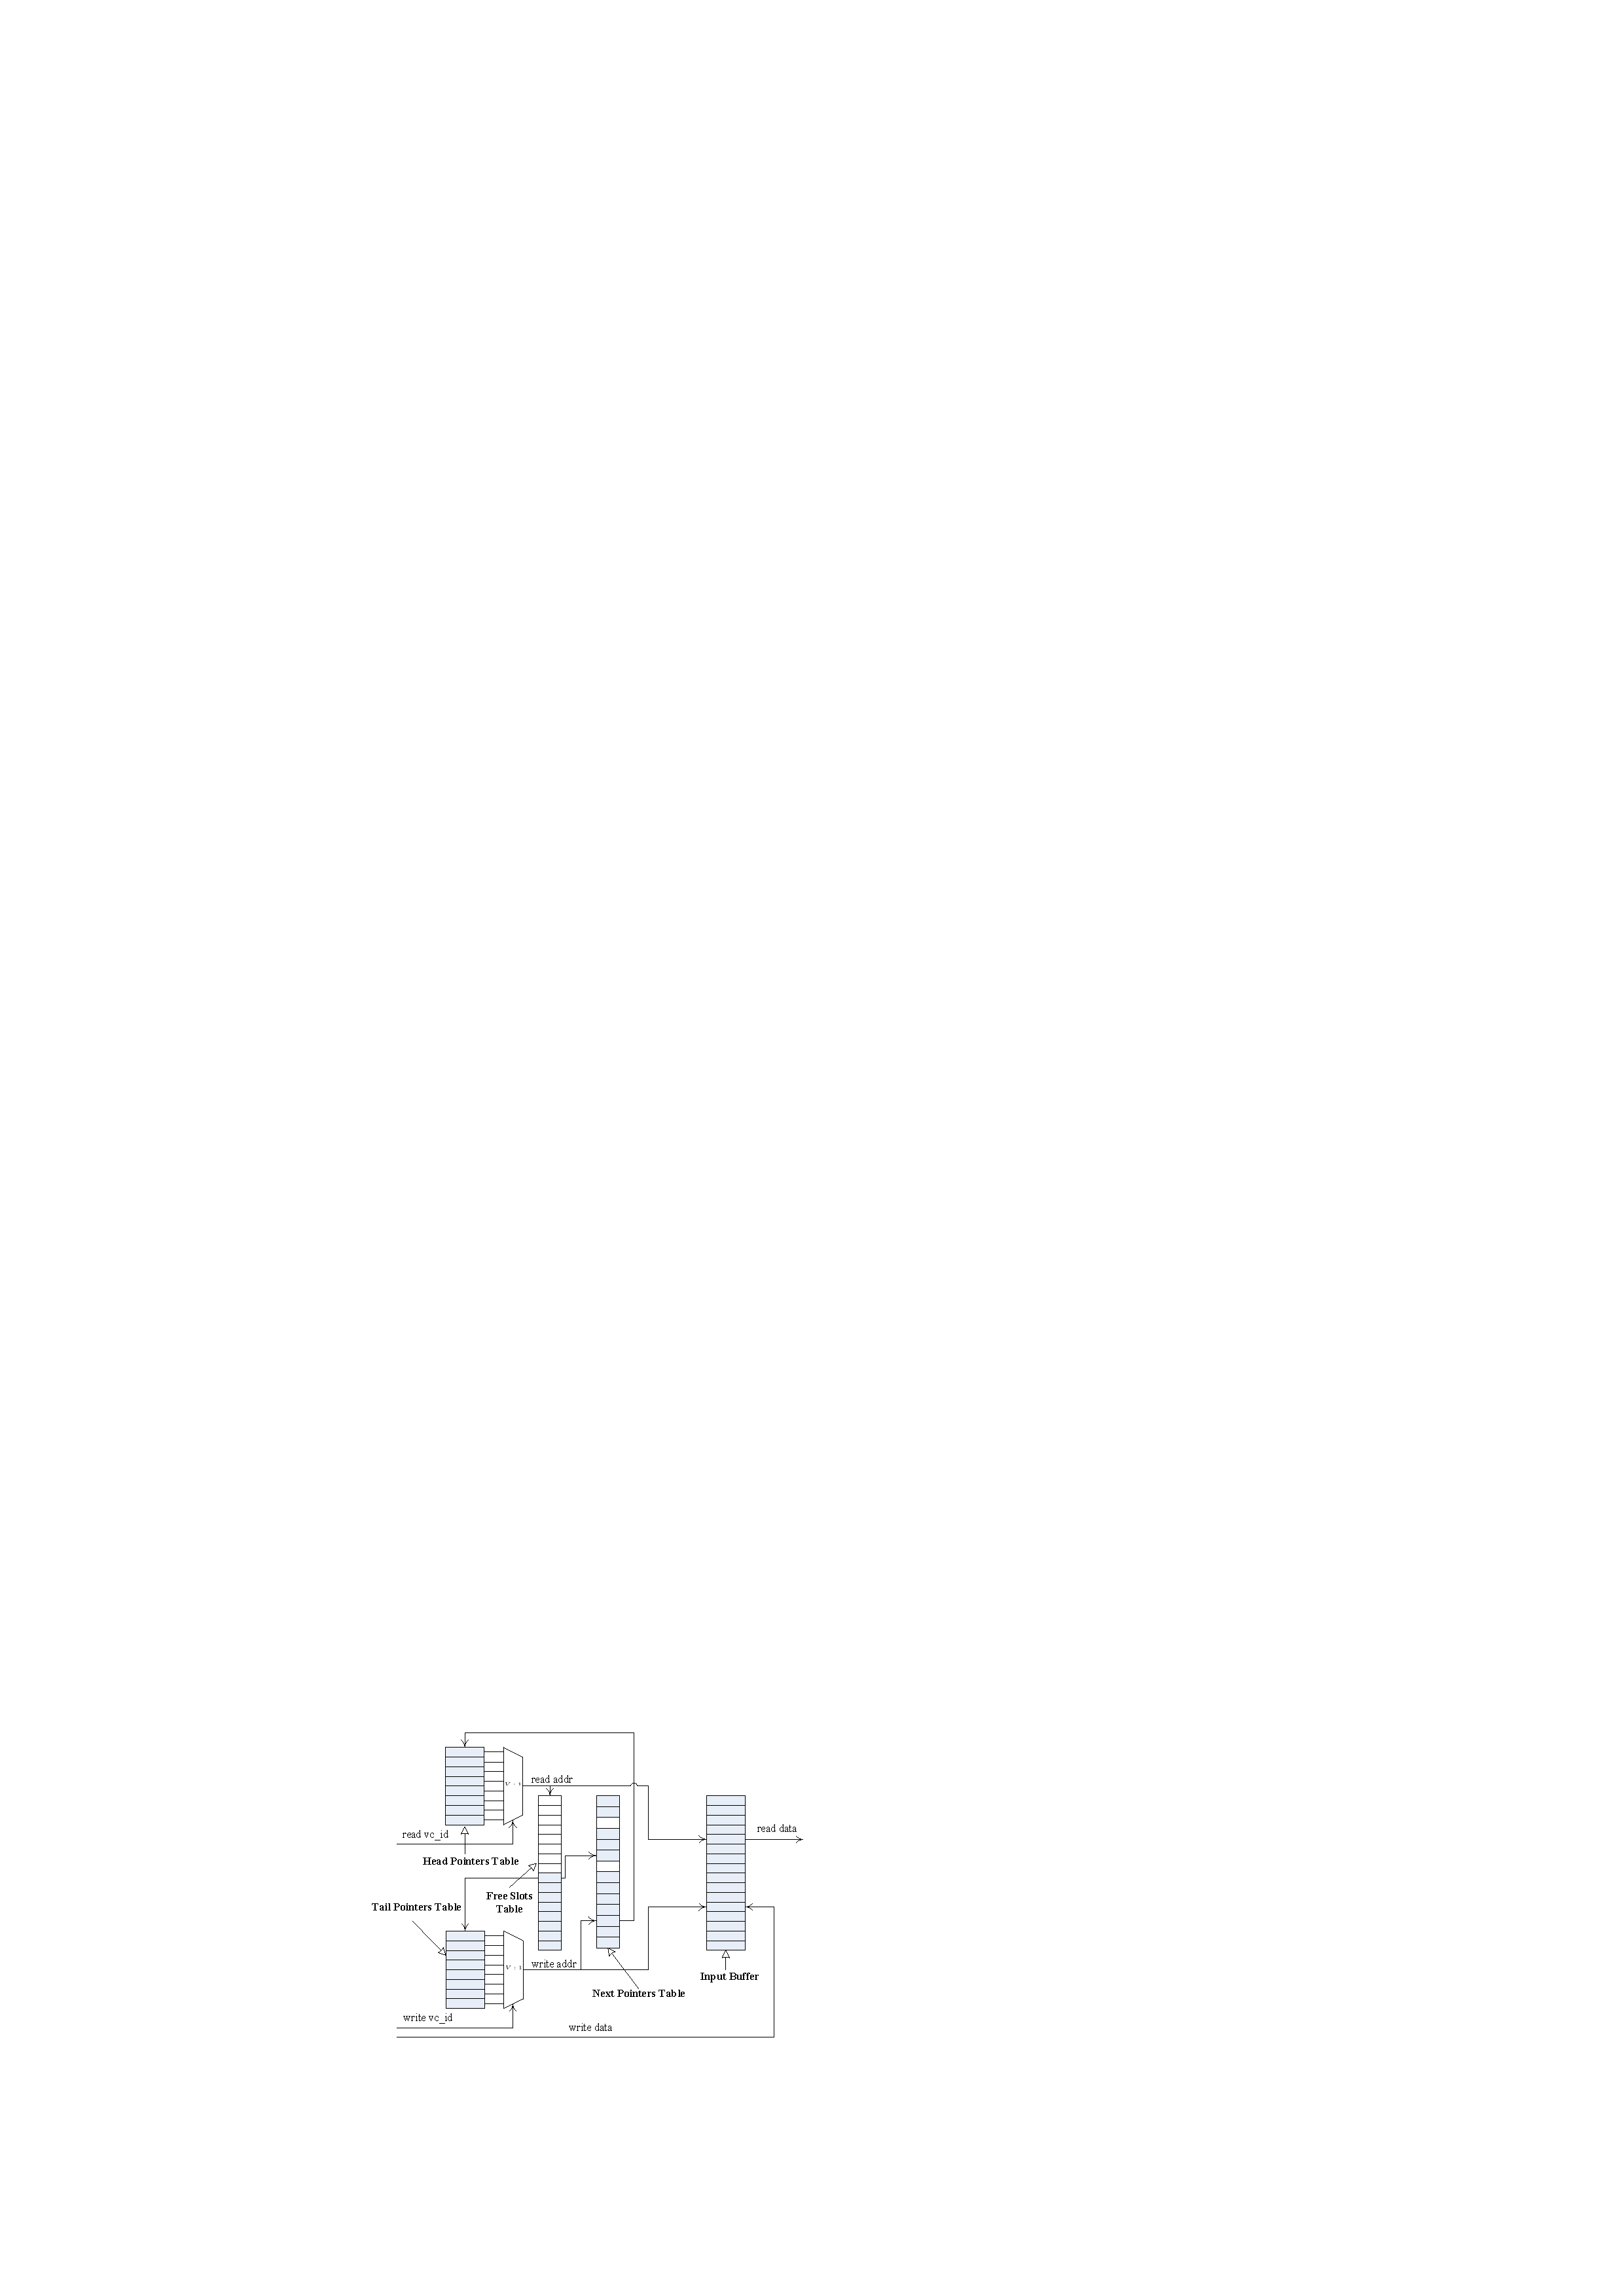
\includegraphics[scale=0.65]{figures/linklist.pdf}\label{linklist}}
  \caption{The proposed AVCS router architecture and the buffer management scheme}
\end{figure*}

After the buffer allocator determines the new owner of shared buffer bank, the allocation results are sent to the upstream routers by raising the \emph{sbuf\_grant} signal. Each output port of neighbor router updates the shared VC state upon receiving the signal. The shared VCs are allocated at the granularity of bank: Only when a shared buffer bank is granted to an input port, the corresponding shared VCs can be utilized by this input port. The SWA schedules the flits located at both shared VCs and private VCs to traverse the crossbar and enter the input port of downstream router. Upon arriving the input port of a router, a flit is written into the shared or private buffer according to the \emph{shared\_vc} signal. Each shared buffer bank utilizes a multiplexer ($\textcircled{5}$ in Fig. \ref{architecture}) controlled by the buffer allocator to select the flits coming from the owner port. Similarly, each input port of the crossbar uses a multiplexer ($\textcircled{6}$ in Fig. \ref{architecture}) controlled by the SWA to select the flits from either private buffer or shared buffers.

The credit-based flow control requires a credit receiving module at the output port of upstream router and a credit generating module at the input port of downstream router. Since the private buffer and shared buffer are managed independently in AVCS router, a dedicated credit counter for each shared buffer bank is necessary. To distinguish whether the credit is for the shared VCs, an additional signal \emph{credit\_for\_shared\_vc} driven by credit generator is connected to the corresponding credit receiver besides the \emph{credit\_valid} and \emph{credit\_value} signal, as shown in Fig. \ref{architecture}.
\begin{comment}
基于信约的流量控制由两部分组成,一部分是位于路由器输出端口处的信约接收模块,一部分是位于下流路由器输入端口中的信约生成模块。信约生成模块则根据交换机仲裁的结果向上游路由器反馈信约,而信约接收模块则会根据反馈的信约来更新信约计数器。在我们的AVCS结构中,由于私有缓存和共享缓存是独立管理的,因此在信约接收模块中除了有一个针对私有缓存的信约计算器以外,还需要为每个共享的存储体设置一个独立的信约计数器。而信约生成模块在反馈信约时还需要标明当前信约是私有信约还是共享信约。如果反馈的是共享信约,那么信约接收模块会根据信约中携带的共享缓存ID更新相应的共享信约计算器。由于信约为零存储体不能接收新的切片,因此信约计算器的值会作为交换机分配的参考。
\end{comment}

To improve the performance with limited buffer resources, we must manage and allocate the buffer resources dynamically according to the traffic condition. Two methods have been proposed to achieve this aim, e.g. UBS \cite{NPKV06}\cite{5770788} and LLS \cite{4555894}\cite{Neishaburi:2009:RAN:1531542.1531658}. Since UBS is only applicable to the fixed-length packet network, we adapt LLB scheme for both shared and private buffer in our approach to increase the buffer utilization. Five tables are necessary to implement LLB scheme, as shown in Fig. \ref{linklist}. A Next Pointers Table records the next slot address for each buffer slot; A Tail Pointers Table maintains the writing address of each VC; A Header Pointers Table keeps the reading address for each VC; A Free Slots Table tracks the address of all the unused buffer slot; In addition, a VC State Table is used to identify the occupied VCs.
\begin{comment}
我们的设计方案是在典型路由器结构的基础增加和共享缓存和一些对共享缓存的控制和分配模块形成的。为了以较少的缓存空间提高典型片上网络的性能,我们必须提高对共享缓存的利用率,这就需要我们能够对路由器内部每个端口以及每个端口中每个虚通道的缓存都进行有效的动态管理和共享。目前两类动态缓存管理方案是UBC\cite{NPKV06}和基于链表\cite{4555894}\cite{Neishaburi:2009:RAN:1531542.1531658}\cite{5770788} 的方式,UBC 只能用于固定报文长度而基于链表的方式则没有这些限制。因此本文采用基于链表的方式来管理both shared memory bank and the private buffer to guarantee the buffer utilization。 基于链表的组织方式需要为每一个buffer slot 增加一个next slot pointer,并为每个虚通道提供一个tail 和head 指针,同时提供一个fifo 结构来跟踪空闲的slot,如图\ref{linklist}所示。
\end{comment}

The main difference between typical router and our proposal lies in the buffer and VC organization, as shown in Fig. \ref{org}. For the same amount of buffer slots $B$ and VC number $V$, each input port of our AVCS router reserves $5/6B$ slots as private buffer and shares $B/6$ slots with other input ports. Meanwhile, the VC resources within the shared buffer bank are shared among all these input ports. The shared buffer can change their owner according to the traffic condition of each input port to improve the buffer utilization and network performance. Under low traffic load, the private buffer and VC resources of each input port is capable of delivering all the incoming traffic. While under high traffic load, the shared buffer and VCs of idle input ports will be designated to the congested port later to alleviate the congestion. The amount of buffer slots each input port can use lies between $5/6B$ and $10/6B$, in contrast to $B$ of typical router. Similarly, the number of VCs each input port can use lies between $5/6V$ and $10/6V$.
\begin{comment}

我们PVCS结构会根据当前路由器每个端口的拥塞情况来动态的调整每个共享存储体所属的端口,在提高缓存利用率的同时最大化网络性能。当负载较轻时,每个端口的私有存储资源和虚通道便足够支持切片的传输。当某个端口发生拥塞时,某个空闲端口所拥有的共享缓存便会在苦干周期之后被重新分配给该端口以缓解拥塞。由于对共享存储模块的分配是与路由器流水线并行工作的,因此不会对对系统的频率产生不利的影响。

\end{comment}
\begin{figure}
  \centering
  \subfloat[AVCS-NoC]{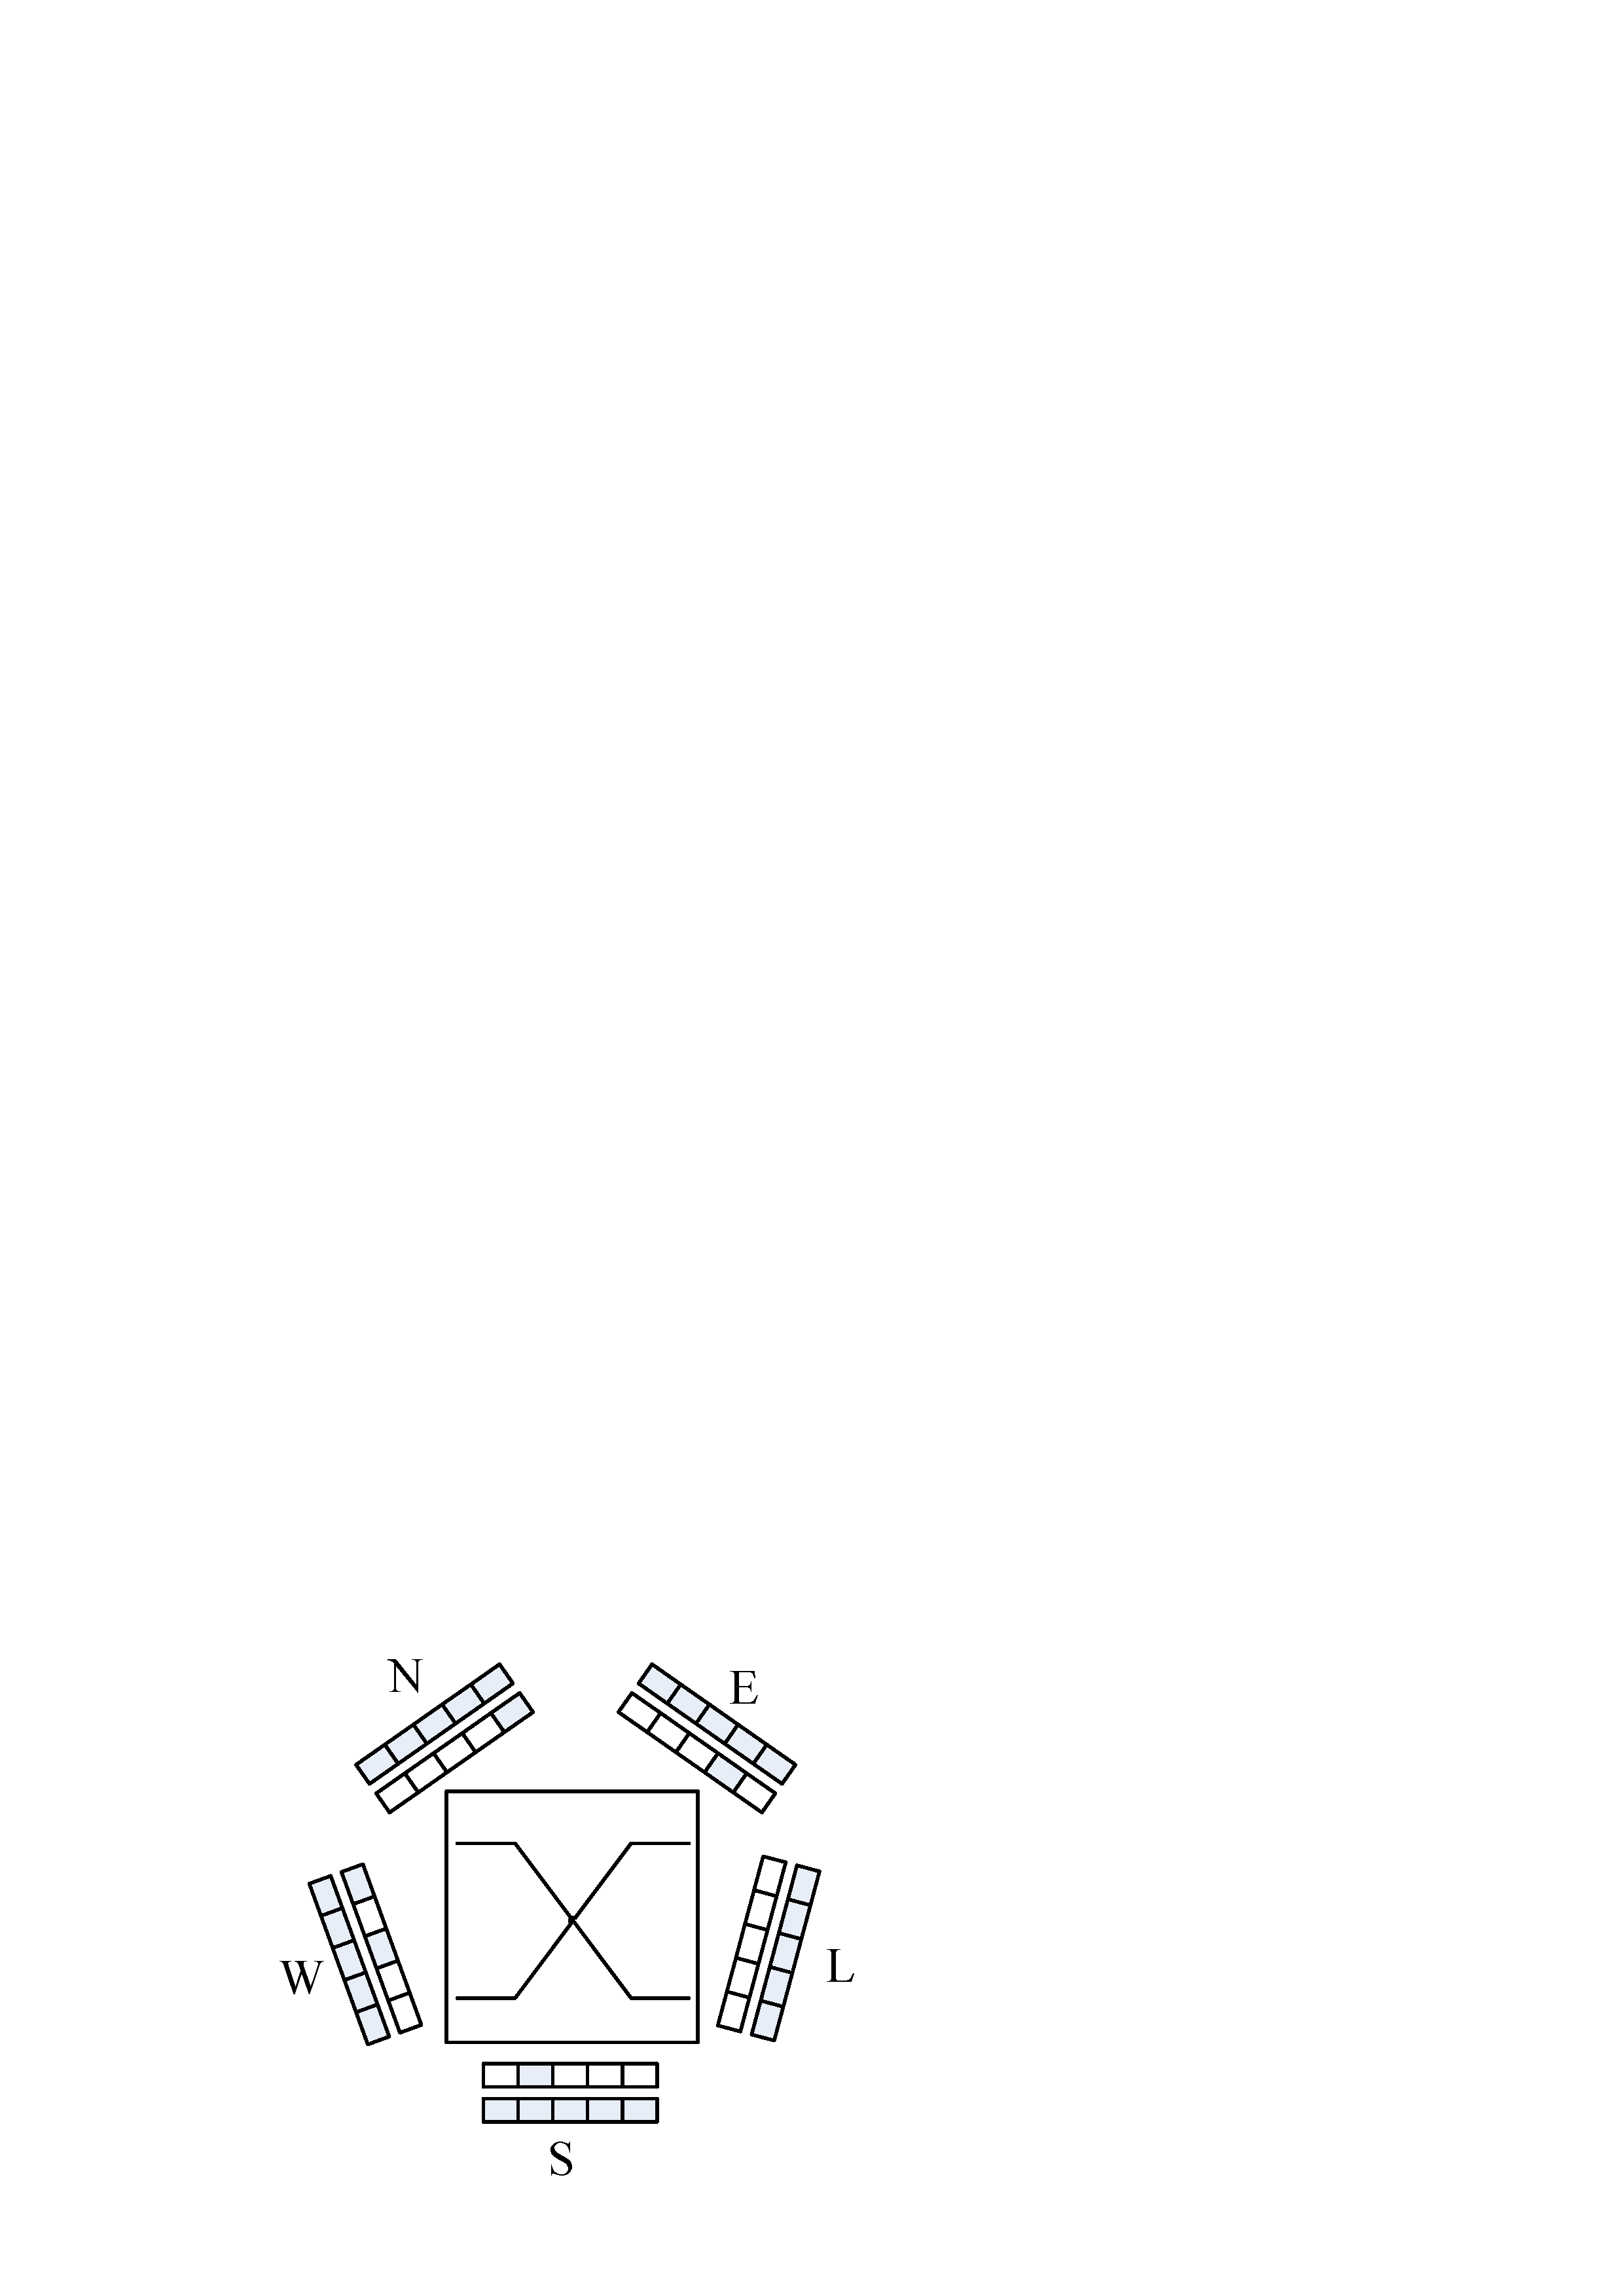
\includegraphics[scale=0.25]{figures/avcsbuf.pdf}\label{avcsbuf}}\hspace{10pt}
  \subfloat[typical router]{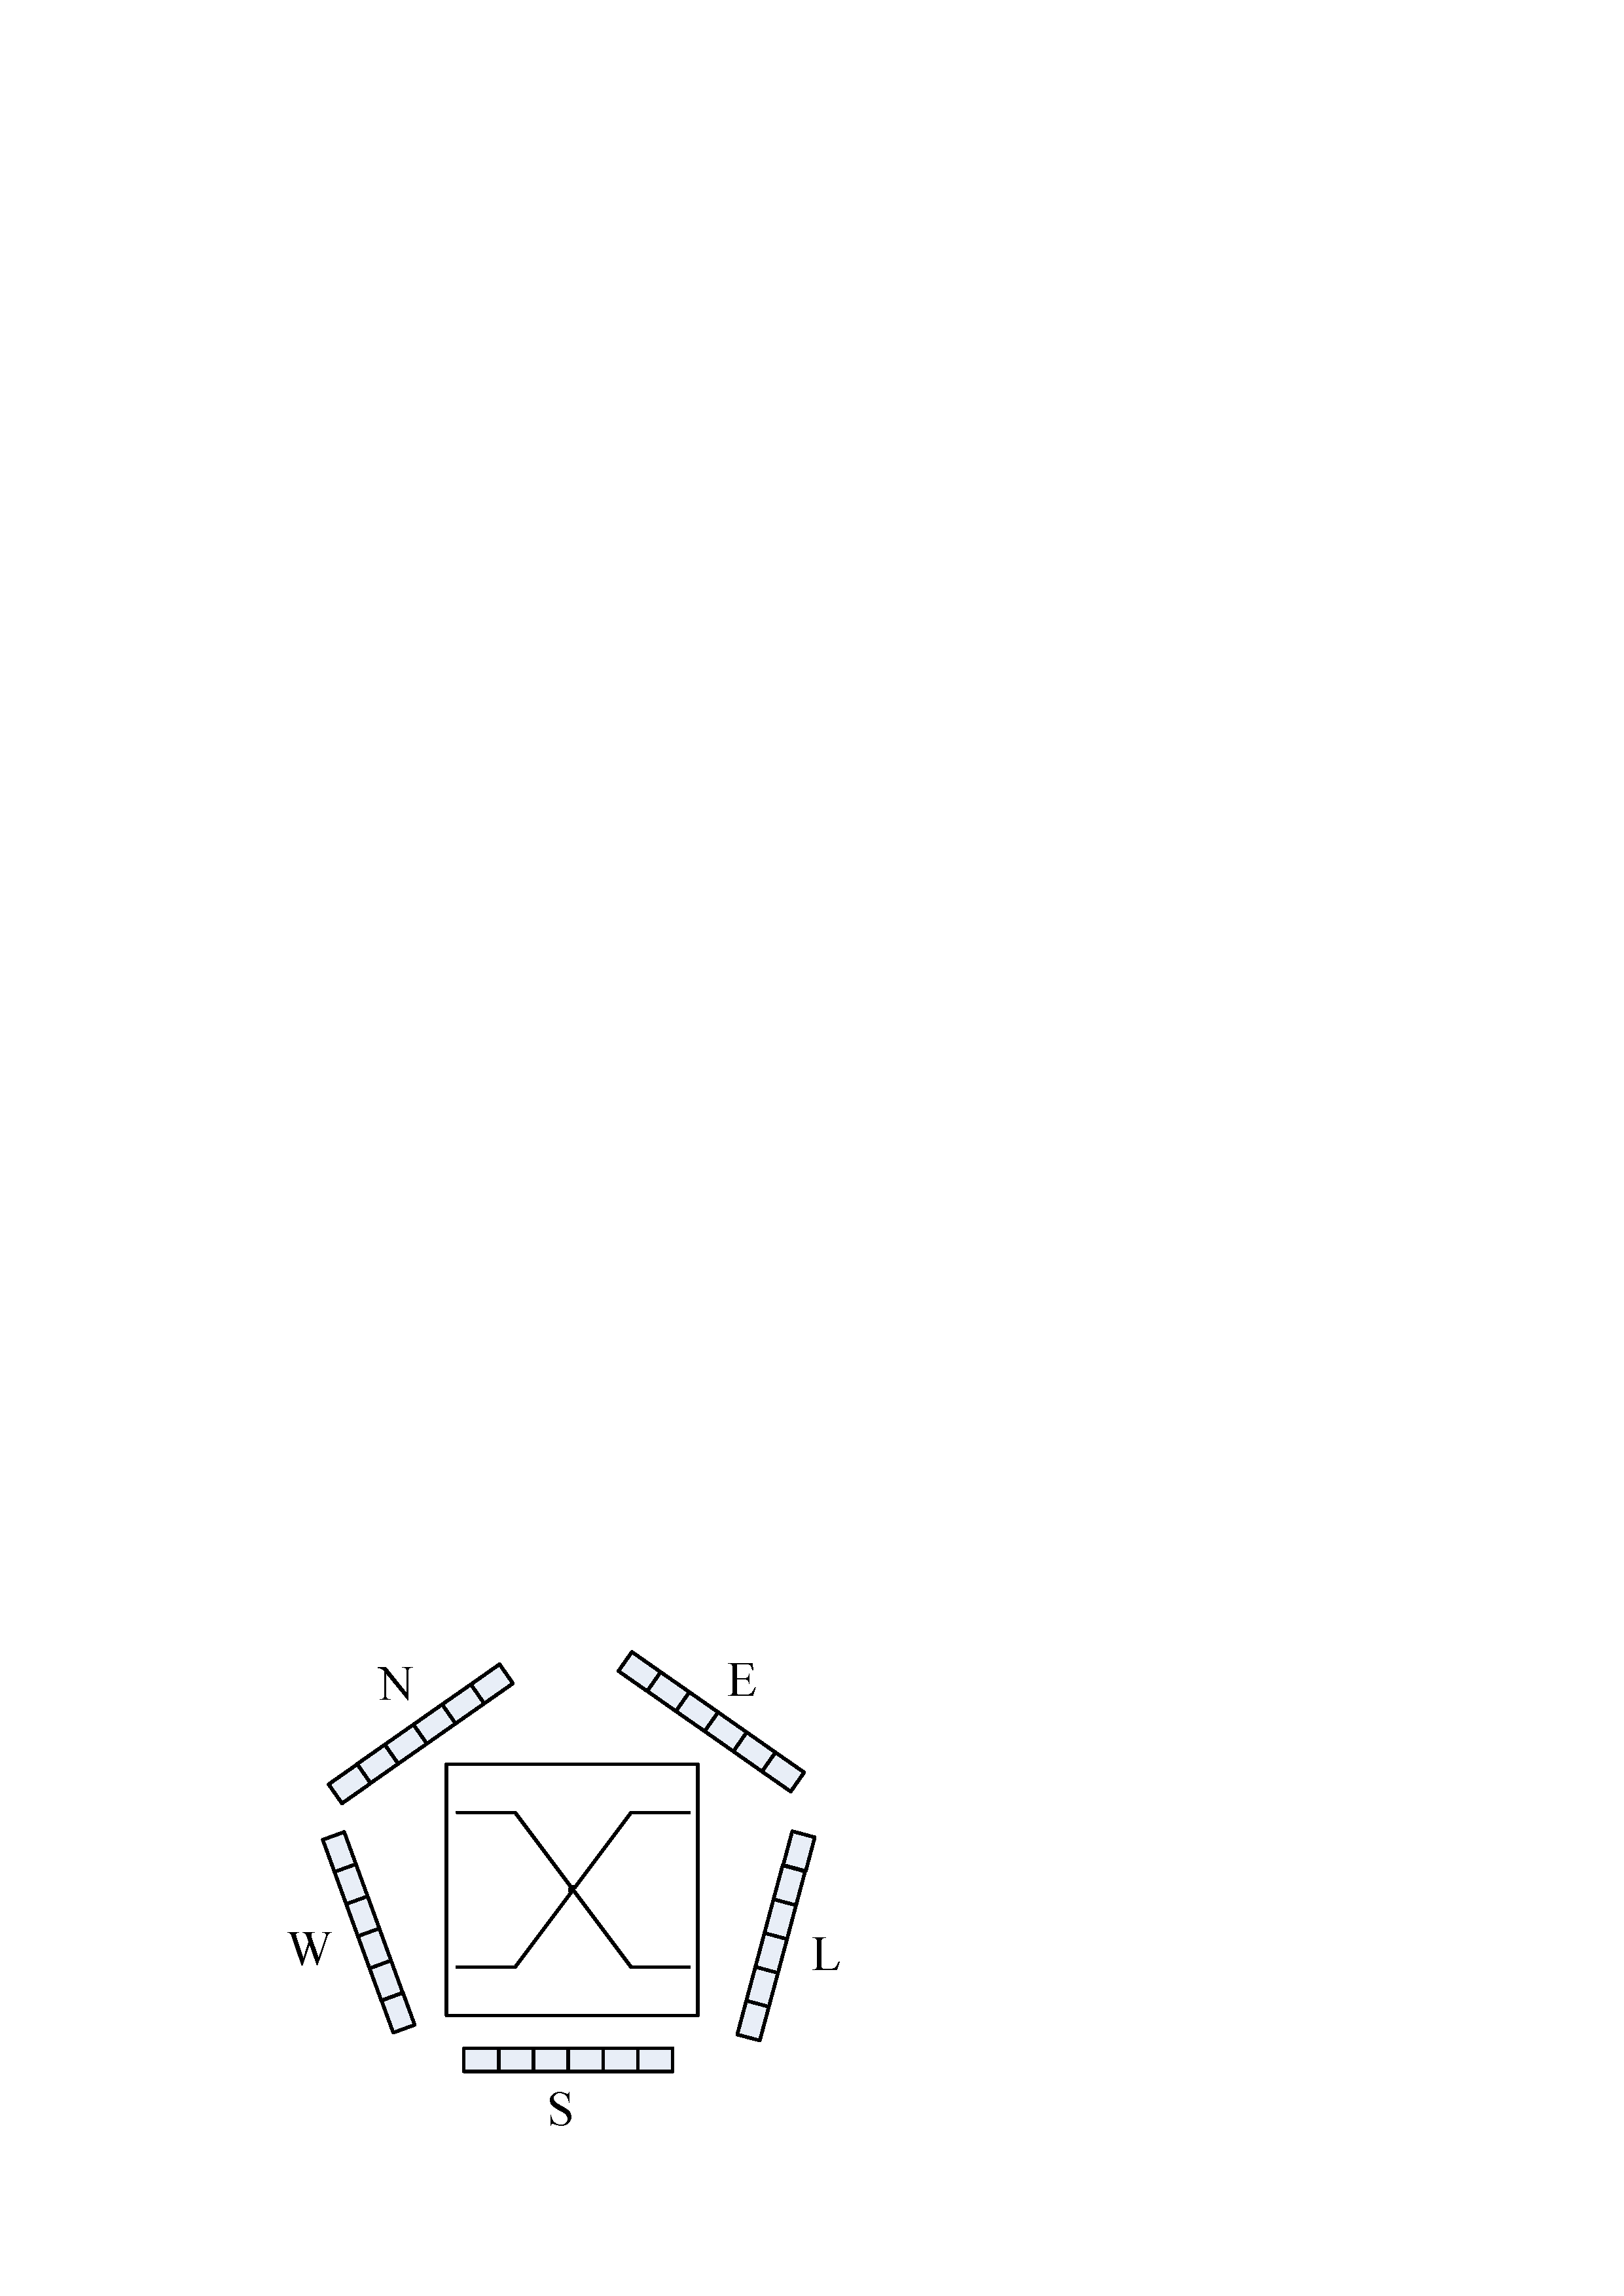
\includegraphics[scale=0.25]{figures/typicalbuf.pdf}\label{typicalbuf}}
  \caption{Buffer organization of AVCS-NoC and typical router.}\label{org}
\end{figure}

Our proposal resolves all the aforementioned questions:
\begin{enumerate}
\item This architecture is a partial buffer and VC sharing scheme, even when all the shared buffer is occupied by some input ports, the other ports can still use their private buffer to guarantee the transmission of packets, which alleviates the interference caused by complete inter-port buffer and VC sharing.
\item The hardware overhead of our proposal is much lower than the fully-shared scheme, e.g. \cite{Neishaburi:2009:RAN:1531542.1531658}\cite{5770788}, which realizes better trade-off between cost and performance. We will discuss this issue in subsection \ref{controllogic}.
\item The shared buffer is divided into several small banks to support parallel access. Each bank can only be granted to one input port at any time, which avoid the multiple read/write conflicts.
\item In order to minimize the complexity and overhead of VCA and SWA, we let the shared VCs and private VCs sharing the same request port, as explained in subsection \ref{allocmux}. This approach makes it possible to arbitrate large amount of VCs by using a smaller VCA and SWA, which reduces the complexity of these two allocators significantly.
\end{enumerate}

In addition, our proposal can withstand the presence of faulty of both private and shared VCs, since a faulty private VC can be replaced by its corresponding non-faulty shared VC, and a faulty shared VC does not interrupt the the functionality of corresponding private VC.
\begin{comment}
将上述几点考虑在内,我们提出了如图\ref{architecture} 所示的自适应端口间缓存和虚通道共享体系结构。该体系结构在路由器端口之间实现了缓存和虚通道的部分共享:每个端口保留一定数量的私有缓存和虚通道,还有一部分共享的缓存和虚通道在运行过程中按需分配给不同的端口使用。我们提出的结构有效的解决了上面提出的4个问题:1. 由于是部分共享的方案,私有缓存和虚通道相当于是为每个端口预留的配额,因而可以有效的缓解共享缓存被某个端口耗尽时对低速端口的干扰,有效的实现了端口间的流量隔离。2. 与完全共享方案相比,部分缓存共享引入的硬件开销较小,很好的实现了性能和成本之间的折衷。3. 我们将共享的缓存分成了若干个相互独立的存储体,每个存储体在任意时间都只能被一个端口使用,因此避免了可能的读写冲突。4. 为了解决分配的规模问题,我们提出了影子虚通道的概念,在不影响性能的情况下,通过分配器的端口复用来实现以较小的分配器实现对大量虚通道的分配和仲裁。之外,我们提出的方案还具有天然的容错特性:当某个端口的某些虚通道发生故障时,共享虚通道可以补充过来代替私有的虚通道进行数据传输。
\end{comment}

The AVCS router architecture is different from the previously proposed ViChaR \cite{NPKV06}, which needs fully re-implement the router pipeline. In contrast, our approach augments typical router architecture \cite{DaTo01} by adding a shared buffer allocator for each shared buffer bank and re-implementing VCA and SWA. The buffer allocator works in parallel with router pipeline, which imposes no negative effect on the critical path of entire router. We will introduce the implementation of buffer allocator, VCA and SWA in the following two subsections.
\begin{comment}
与之前基于UBS的方案不同,我们的体系结构不需要对整个路由器流线进行重新设计,而是在经典路由器体系结构的基础上增加以下几个模块而形成的:1. 共享buffer 的分配和管理模块:负责对共享缓存和虚通道的分配与释放,读写地址和控制信号的译码以及队列空满检测模块,我们将在第
\ref{bufmanage}小节进行介绍; 2. 虚通道和交换机的仲裁模块,负责在影子vc 和实际vc 之间的仲裁和分配,我们将在\ref{allocmux} 小节进行介绍;3. 共享存储体的流量控制模块:负责跟踪共享存储体的使用、生成信约和流量控制信号,我们将在第\ref{flowctrl}小节对该模块进行详细的介绍。
\end{comment}

\subsection{Shared Buffer Allocation Module}\label{bufmanage}
The shared buffer allocator in our AVCS router is an FSM, which has three states: Enable\_Allocation(EA), Disable\_Allocation(DA) and Change\_Allocation(CA), as shown in Fig. \ref{allocFSM}. The \emph{ready\_for\_allocation} signal keeps on valid while in Enable\_Allocation state. In this state, the shared buffer and VCs can be used by the input port indicated by the \emph{sbuf\_grant} signal. We say that a shared buffer bank is idle when it is empty and no output VC of upstream router was designated to it. When the shared buffer bank keeps on idle for $K$ cycles, we can infer that this input port does not need this bank temporally. Thus, we can reallocate it to other input ports which require more buffer and VC resources. The threshold $K$ is a design parameter, which affects the allocation results and the performance of entire network. For a real-world application, the optimal $K$ can be chosen by experiments. To avoid the shared buffer is reallocated while changing status, the FSM first enters the Disable\_Allocation state. At this state, the \emph{ready\_for\_allocation} signal goes down to disable the output VC allocation at upstream router. When the shared buffer bank is empty and no shared VCs on this bank are allocated, the FSM enters the Change\_Allocation state. At this state, the buffer allocator chooses the new owner for the shared buffer according to the congestion status of each input port and the current owner of this bank (indicated by \emph{sbuf\_grant}), as described in Alg. \ref{alg:bufferalloc}. Then, the FSM enters Enable\_Allocation state and begins another allocation period.
\begin{comment}
在我们提出的AVCS结构中,共享的buffer分成5个或是5的整数倍个bank,用以支持动态的VC分配和端口间的缓存调整。由于每个存储体都独立寻址,因此在同样的缓存容量情况下,我们的方案较UBC\cite{NPKV06}和基于链表
\cite{4555894}\cite{Neishaburi:2009:RAN:1531542.1531658}\cite{5770788} 方式更加节省控制存储空间,我们将在\ref{controllogic} 节通过比较来展现这一优势。我们对vc的分配以存储体为粒度,当某个存储体被分配给相应的端口后,这个存储体上所有的vc也相应的分配给该端口。为了支持这一改变,我们的方案中每个共享的bank 输出5根线用于表示当前bank 授权给评谁用。在路由器的每个输出端口上也有5根线用于表示这5个bank 在该端口的可用性。每个存储体都有一个独立的缓存分配器,通过对各个输入端口的缓存和虚通道占用情况进行监视,根据一定的策略动态的将空闲的bank 分配给指定的比较忙碌的端口使用。在具体的实现过程中,我们可以动态的改进对指定Memory bank 采用的控制策略,以适应不同流量模式的特点并提高其吞吐率。缓存分配器是一个有限状态机,状态机有3 个状态,Enable\_Allocation(EA), Disable\_Allocation(DA)和Change\_Allocation(CA),如图\ref{allocFSM} 所示。
\end{comment}
\begin{comment}
当处于enable allocation 状态时,Ready\_for\_Allocation(RA)信号有效,相应的存储体可以被相应的端口使用。当连续K个周期该共享存储体上所有的VC 都没有被分配而且共享缓存为空时,则认为当前端口暂时不需要该存储体,此时可以将该存储体重新分配给其它端口使用。阈值K是AVCS结构的一个额外的参数,它会影响共享存储体在各个端口之间的分布并最终对性能产生影响。在实际使用时,对于特定的应用可以通过实验来确定最佳的K值。为了防止在状态切换过程中被分配,有限状态机先进入disable allocation 状态,在该状态下向上游路由器发出unready for allocation信号,并在队列为空且虚通道没有被分配时进入下一个状态change allocation。在这个状态下,缓存分配器根据每个端口的拥塞情况按照轮转的方式选择下一个可以使用该存储的端口,选择下一下端口的算法如Alg.\ref{alg:bufferalloc}所示。在完成缓存分配后,状态机进入enable allocation状态。
\end{comment}
\begin{figure}[htb]
  \begin{minipage}[b]{0.3\textwidth}
    \centering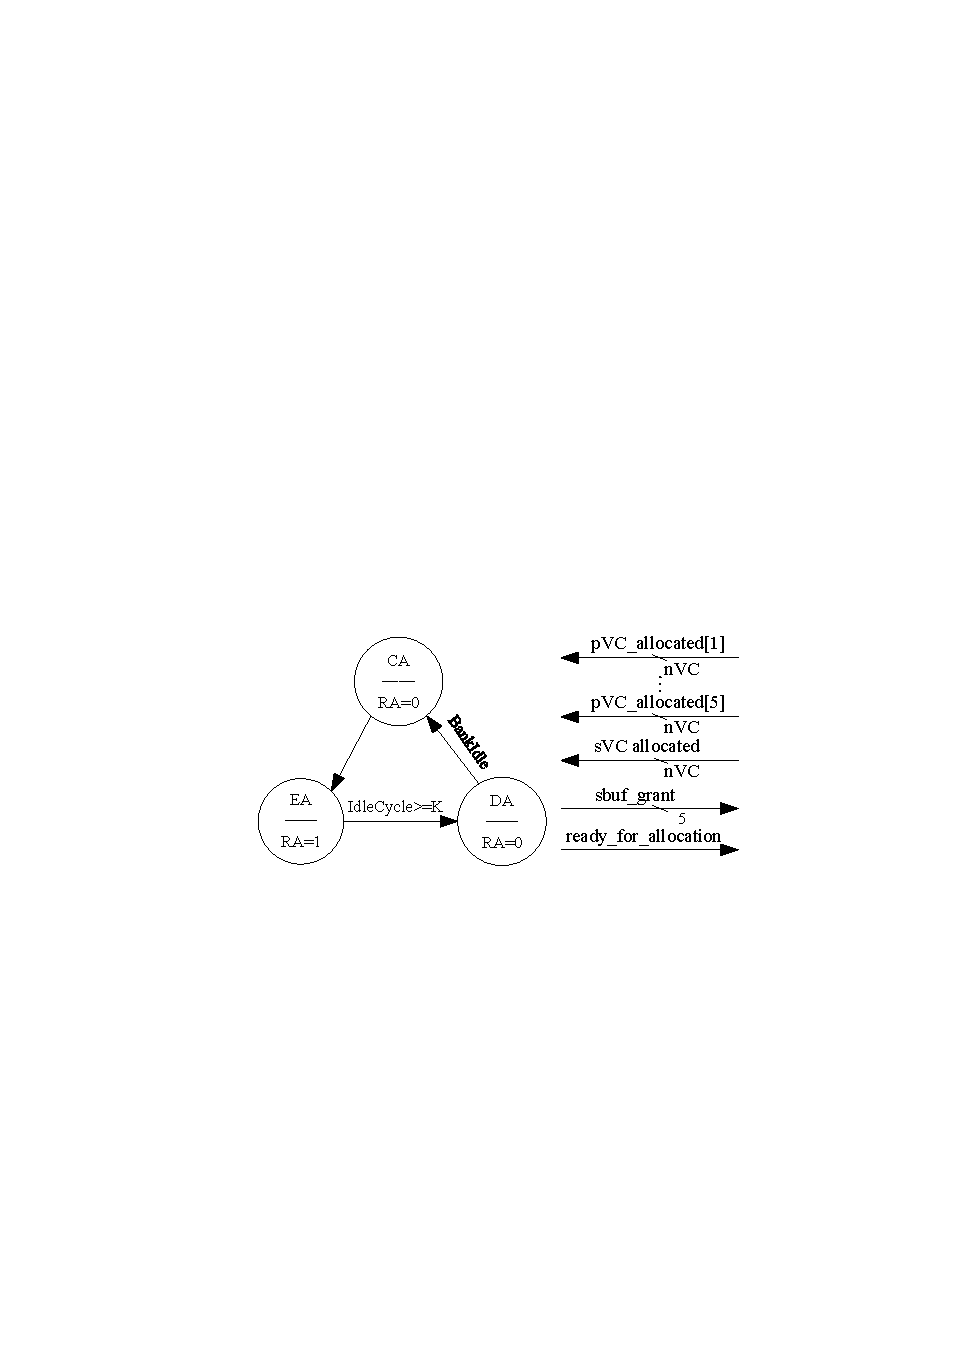
\includegraphics[scale=0.6]{figures/allocFSM.pdf}
    \caption{The FSM of buffer allocator}\label{allocFSM}
  \end{minipage}%
  \begin{minipage}[b]{0.2\textwidth}
    \centering
    \begin{tabular}{|c|c|}
      \hline
      Port & Encode \\
      \hline\hline
      East  & 10000 \\
      \hline
      West    & 01000 \\
      \hline
      South &   00100\\
      \hline
      North & 00010\\
      \hline
      Local & 00001\\
      \hline
    \end{tabular}
    \caption{Port Encoding}\label{portencode}
  \end{minipage}
\end{figure}

To simplify the allocation algorithm, we choose the owner of each shared buffer bank in round-robin order. This is achieved by using a five-bit register \emph{port\_mask} to filter out the ports can not be chosen as candidate at current allocation period (Step 4 and Step 7). Initially, these five buffer banks belongs to different input ports (Step 3 and Step 6). When the FSM enters Change\_Allocation state, the five-bit \emph{port\_busy} (generated in Step 11) and \emph{port\_mask} registers are used to determine the new owner of this bank (Step 13 to 21). The fundamental idea of this algorithm is that choosing the candidate in order and skip the idle input ports to accelerate this process. If the position of the left-most `1' in the selector signal (generated at Step 13) matches one of the input ports listed in Fig. \ref{portencode}, the shared buffer is granted to this port. The encoding scheme also indicates that the choosing order of this algorithm is: East $\to$ West $\to$ South $\to$ North $\to$ Local $\to$ East. One example of how this algorithm functions is illustrated in Fig. \ref{Algorithm}. For a real-world application, we can also change the allocation algorithm to adapt the characteristic of traffic pattern.
\begin{algorithm}
\caption{Shared buffer allocation}\label{alg:bufferalloc}
\begin{algorithmic}[1]
\STATE \textbf{Initialized:}
\STATE \ \ \ \ \textbf{if}(bank\_id==5)
\STATE \ \ \ \ \ sbuf\_grant = 5'b00001;
\STATE \ \ \ \ \ port\_mask = 5'b11111;
\STATE \ \ \ \ \textbf{else}
\STATE \ \ \ \ \ sbuf\_grant = East $>>$ bank\_id;
\STATE \ \ \ \ \ port\_mask = 5'b11111 $>>$ (bank\_id+1);
\STATE \ \ \ \ \textbf{endif}
\STATE \textbf{Change\_Allocation:}
\STATE \ \ \ \ \textbf{for}(p=1;p$<=$5;p=p+1)
\STATE \ \ \ \ \ port\_busy[p] = $|$ pVC\_allocated[p];
\STATE \ \ \ \ \textbf{endfor}
\STATE \ \ \ \ selector = port\_mask \& port\_busy;
\STATE \ \ \ \ \textbf{case}(selector)
\STATE \ \ \ \ \ \ \ \ 5'b1xxxx: sbuf\_grant = East; port\_mask=5'b01111;
\STATE \ \ \ \ \ \ \ \ 5'b01xxx: sbuf\_grant = West; port\_mask=5'b00111;
\STATE \ \ \ \ \ \ \ \ 5'b001xx: sbuf\_grant = South; port\_mask=5'b00011;
\STATE \ \ \ \ \ \ \ \ 5'b0001x: sbuf\_grant = North; port\_mask=5'b00001;
\STATE \ \ \ \ \ \ \ \ 5'b00001: sbuf\_grant = Local; port\_mask=5'b11111;
\STATE \ \ \ \ \ \ \ \ default: port\_mask=5'b11111;
\STATE \ \ \ \ \textbf{endcase}
\end{algorithmic}
\end{algorithm}
\begin{figure}
\centering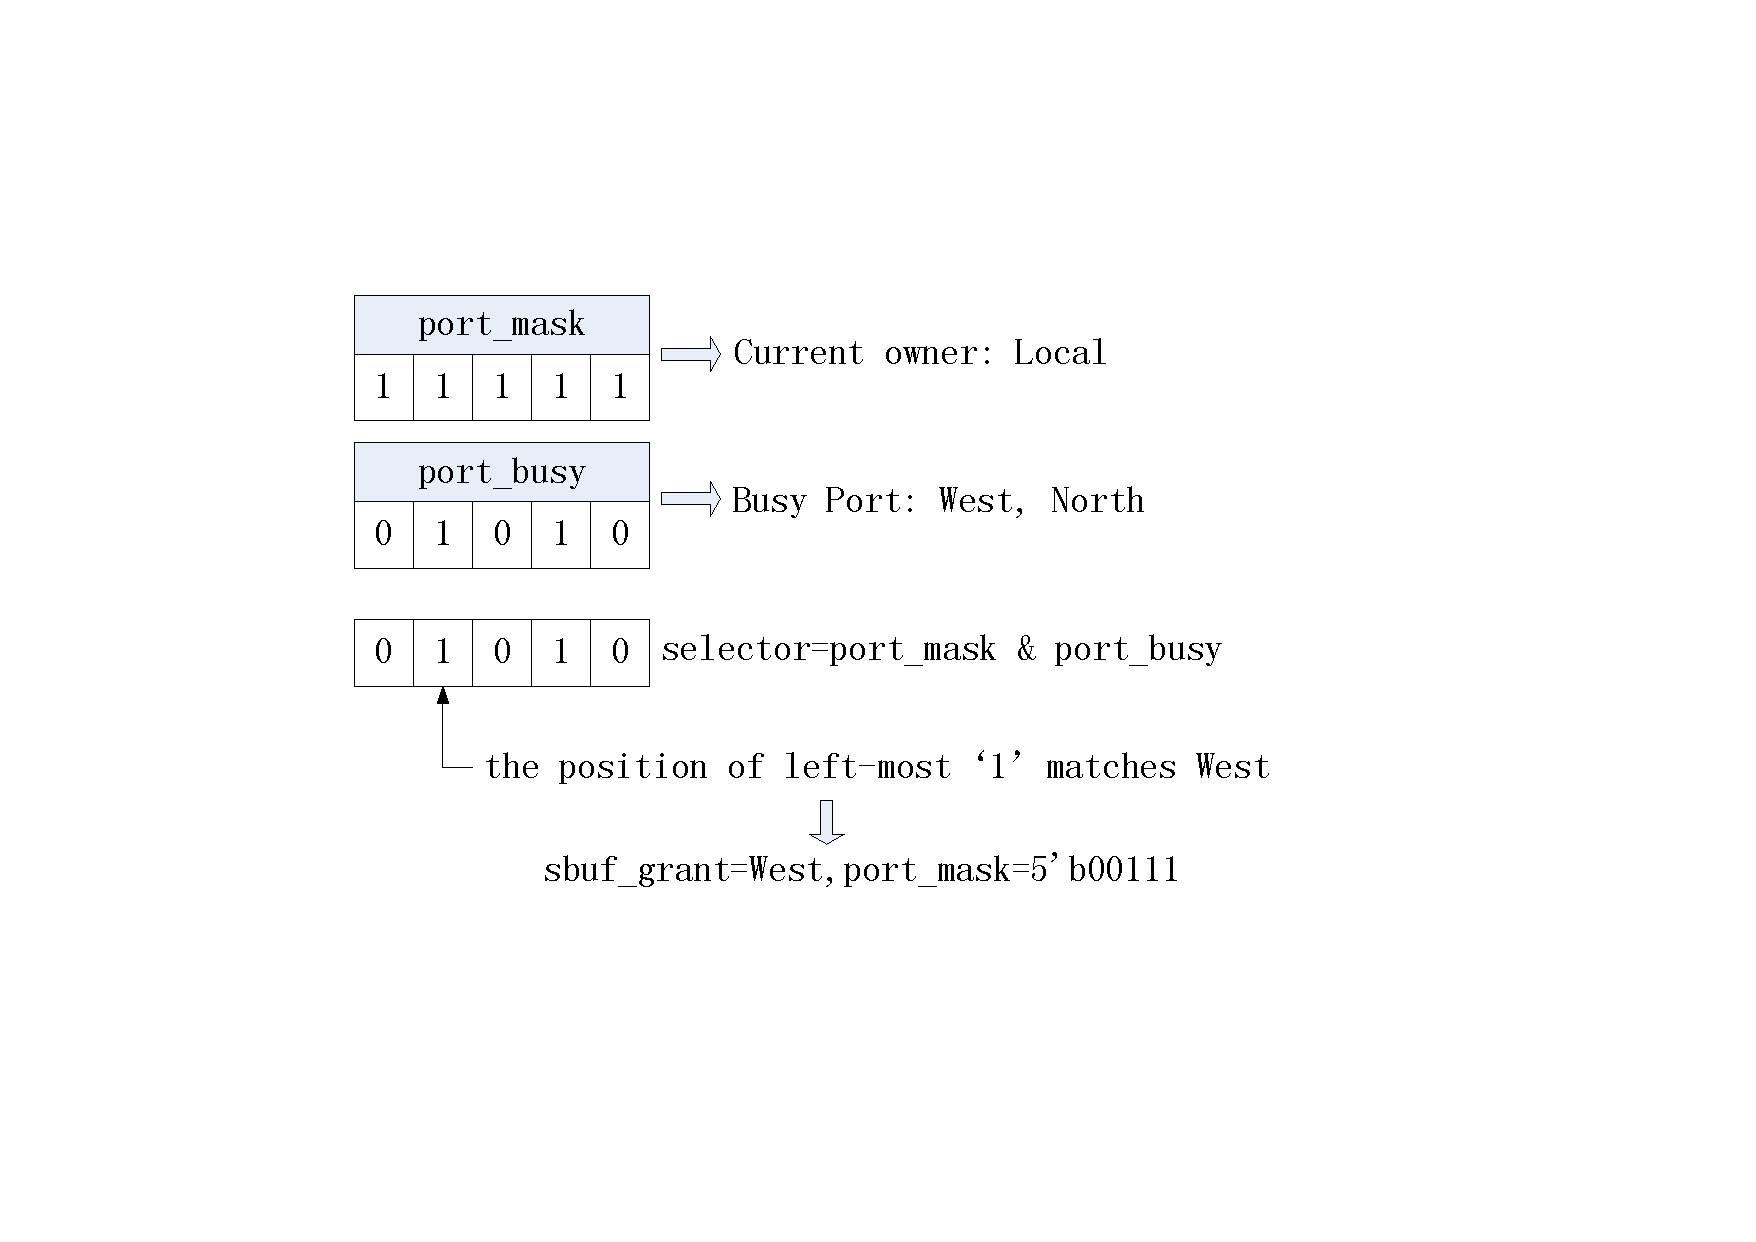
\includegraphics[scale=0.5]{figures/Algorithm.pdf}
\caption{A step-by-step example of buffer allocation algorithm}\label{Algorithm}
\end{figure}

\subsection{VC and SW Allocator}\label{allocmux}
The goal of inter-port buffer and VC sharing is to alleviate the performance degradation caused by flow control and VC blocking. Because the allocation results changes with traffic load, our architecture is more suitable to address the blocking caused by unbalanced VC and buffer requirement of different input ports. The VCs each input port can use in AVCS router includes the private VCs owned by this port and the VCs shared among all the ports. Thus, the number of VCs each input port can use varies with traffic condition, since an input port with heavy traffic load is likely to own more shared buffer banks. Denote the number of input ports and the maximal shared VCs (including private and shared VCs) each input port can use as $P$ and $V_{max}$. The VCA matches $P\times V_{max}$ requests from $P$ input ports with $P\times V_{max}$ output VCs. Similarly, the SWA matches the $P\times V_{max}$ request from $P$ input ports to $P$ output ports. To support the worst-case VC and switch allocation, one solution is that by adapting a $PV_{max}\times PV_{max}$ VCA and a $PV_{max}\times P$ SWA. However, this makes these two allocators complex and introduce significant hardware overhead.
\begin{comment}
采用端口间的VC共享方案的根本目的是为了尽可以避免VC阻塞造成的性能下降。由于实现了VC共享,在我们提出的路由器结构中,每个端口所能使用的虚通道有两个部分组成:一部分是每个端口的私有虚通道;另一部分是在各个端口间共享的虚通道。只有当某个存储体被分配给某个端口后,相应的vc 才能够被该端口使用。因此,每个端口所能使用的虚通道的数量是动态变化的。记端口数量为P,每个端口所能使用的最大的虚通道数量为$V_{max}$。 为了支持对最差情况下的虚通道分配和交换机分配,一种可选的方法是为每个路由器配置一个$PV_{max}\times PV_{max}$的虚通道分配和一个$PV_{max}\times P$ 的交换机分配器。但是,这样会使得整个系统变得非常复杂而且还会限制系统所能达到的时钟频率。因此在本文中我们采用另一种方法。
\end{comment}

In this paper, we employ another approach. Our approach lies on two properties of AVCS router: (1) The maximum number of shared VCs in AVCS-NoC is equal to the number of private VCs owned by each input port, and (2) the minimum number of shared VCs each input port can use is zero. Thus, the actually available VCs of each input port can use lies between $1/2V_{max}$ and $V_{max}$. We assign an unique ID to each shared VC, and let these shared VCs compete for the request ports with private VCs. Then, we can use a $1/2PV_{max}\times 1/2PV_{max}$ VCA and a $1/2PV_{max}\times P$ SWA to perform the VC and switch allocation. The reason we employ a smaller VCA and SWA with port sharing rather than a larger allocator lies in the fact that the port utilization of VCA and SWA is very poor, especially for the VCA, as demonstrated in Fig. \ref{utilization}. This is because only the head flit of a packet can issue an VC allocation request and the corresponding request port will keep on idle until the tail flit departure from this VC. The idle request port can be reused to improve the utilization.
\begin{comment}
我将为5个共享存储体上的所有vc进行统一的编号,使得每个共享vc都有不同的ID,而且共享vc的总数恰好等于每个端口的私有vc的数量。我们并不为这些共享vc预留专用的分配器端口,而是让这些虚通道复用私有vc的分配器端口,我们称那些共享缓存虚通道为“影子vc”。我们的方案中影子vc与端口的私有vc共享同一个sw端口和va端口,这样既实现支持了大规模vc又降低了功耗和成本。我们将在第\ref{experiemnts}节通过实验来验证这一点。对于之前的共享VC方案,假设原来的动态VC方案中每个端口有x个VC,那么我们的方案每个端口设置5x/6个私有VC,另外还有5x/6个VC 为各个端口间共享的。由于实现了端口间的vc共享,每个路由器端口所能使用的vc数量在5x/6和10x/6之间动态变化,远远大于之前的设计方案. 每个共享输出虚通道都有对应的elig标志位,只有当下游节点相应的memory bank分配给该端口而且相应的vc没有被分配时,该标志位为1,VCA据此来屏蔽不能使用的输出VC。这在一定程度上也缓解了因为vc 分配失败所带来的开销。
\end{comment}
\begin{comment}
需要说明的是,这种端口复用的方法并不会影响网络的性能。对于虚通道分配器来说,一个已经被分配的输入VC在尾切片没有到达之前是不会再发出任何请求的,在此期间该分配器端口可以被影子vc所使用。对于sw分配器来说,如果相应vc的报文因为某些原因被阻塞,那么这个分配器端口也会空闲,此时如果共享vc被分配在这个端口,那么就可以利用这些空闲的分配器端口进行数据传输。由于每个时钟周期每个端口最多输出1个切片,因此只要能够保证每个时钟周期有一个输入虚通道被授权,就可以保证吞吐率,多余的请求在当前周期内是不会被grant的。实现了端口复用之后,每个分配器端口的利用率都大幅度提高,而且报文长度越长,效果就越明显。
\end{comment}

Specifically, when a shared buffer is designated to an input port, the \emph{elig\_svc} flags of all the corresponding shared VCs are asserted to allow the granting of a request. To enable the sharing of request port, we add a $2:1$ selector to each request port to choose a request from either private VC or shared VC, as shown in Fig. \ref{vcallocator}. This selector chooses these two input VCs in round-robin order to prevent livelock. Then a $1/2PV_{max}\times 1/2PV_{max}$ separable input-first allocator \cite{DaTo04} is used to perform the subsequent arbitration. The separable input-first allocator employs $1/2V_{max}$ $1/2V_{max}:1$ arbiters at each input port to grant at most 1 output VC to this request port, and each output port uses $1/2V_{max}$ $1/2PV_{max}:1$ arbiters to select one input request for each output VC. In order to make the allocation of shared buffer sensitive to the dynamical change of traffic, we assign lower priority to the shared output VC. A shared output VC is allocated only when all the private VCs have been occupied. In contrast, to meet the same arbitration demand, the separable input-first allocator used in the typical router needs $V_{max}$ $V_{max}:1$ arbiters to guarantee each input VC can only request at most 1 output VC, and each output port employs $V_{max}$ $PV_{max}:1$ arbiters to grant each output VC to an unique input VC.
\begin{comment}
对于同样的最大虚通道数量$V_{max}$,虚通道分配器的作用是为$P\times V_{max}$个输入请求分配$P\times V_{max}$ 个输出虚通道。如果不采用影子vc技术,需要在每个输入端口采用$V_{max}$个$V_{max}:1$仲裁器用来保证每个输入vc 只能请求1个输出vc,在每个输出端口采用$V_{max}$个$PV_{max}:1$ 仲裁器用来保证每个输出vc只能分配给$PV_{max}$个输入vc中的1个。对于我们采用了影子vc的方案,每个输入端口只需要$5V_{max}/6$ 个$5V_{max}/6:1$ 仲裁器和$2:1$的优先级仲裁器,每个输出端口需要$5V_{max}/6$个$5PV_{max}/6:1$的仲裁器。因此,我们的方案只需要规模为$5/6V_{max}\times 5/6V_{max}$ 的分配器,采用较小的分配器的好处是降低硬件复杂度并易于降低分配器的功耗和面积。为了使得共享vc尽快适应每个端口流量的变化情况并简化共享VC的分配逻辑,我们在Vc分配时为共享vc分配较低的优先级,只有当私有vc全部被占用时才会使用影子vc。
\end{comment}
\begin{figure}
\centering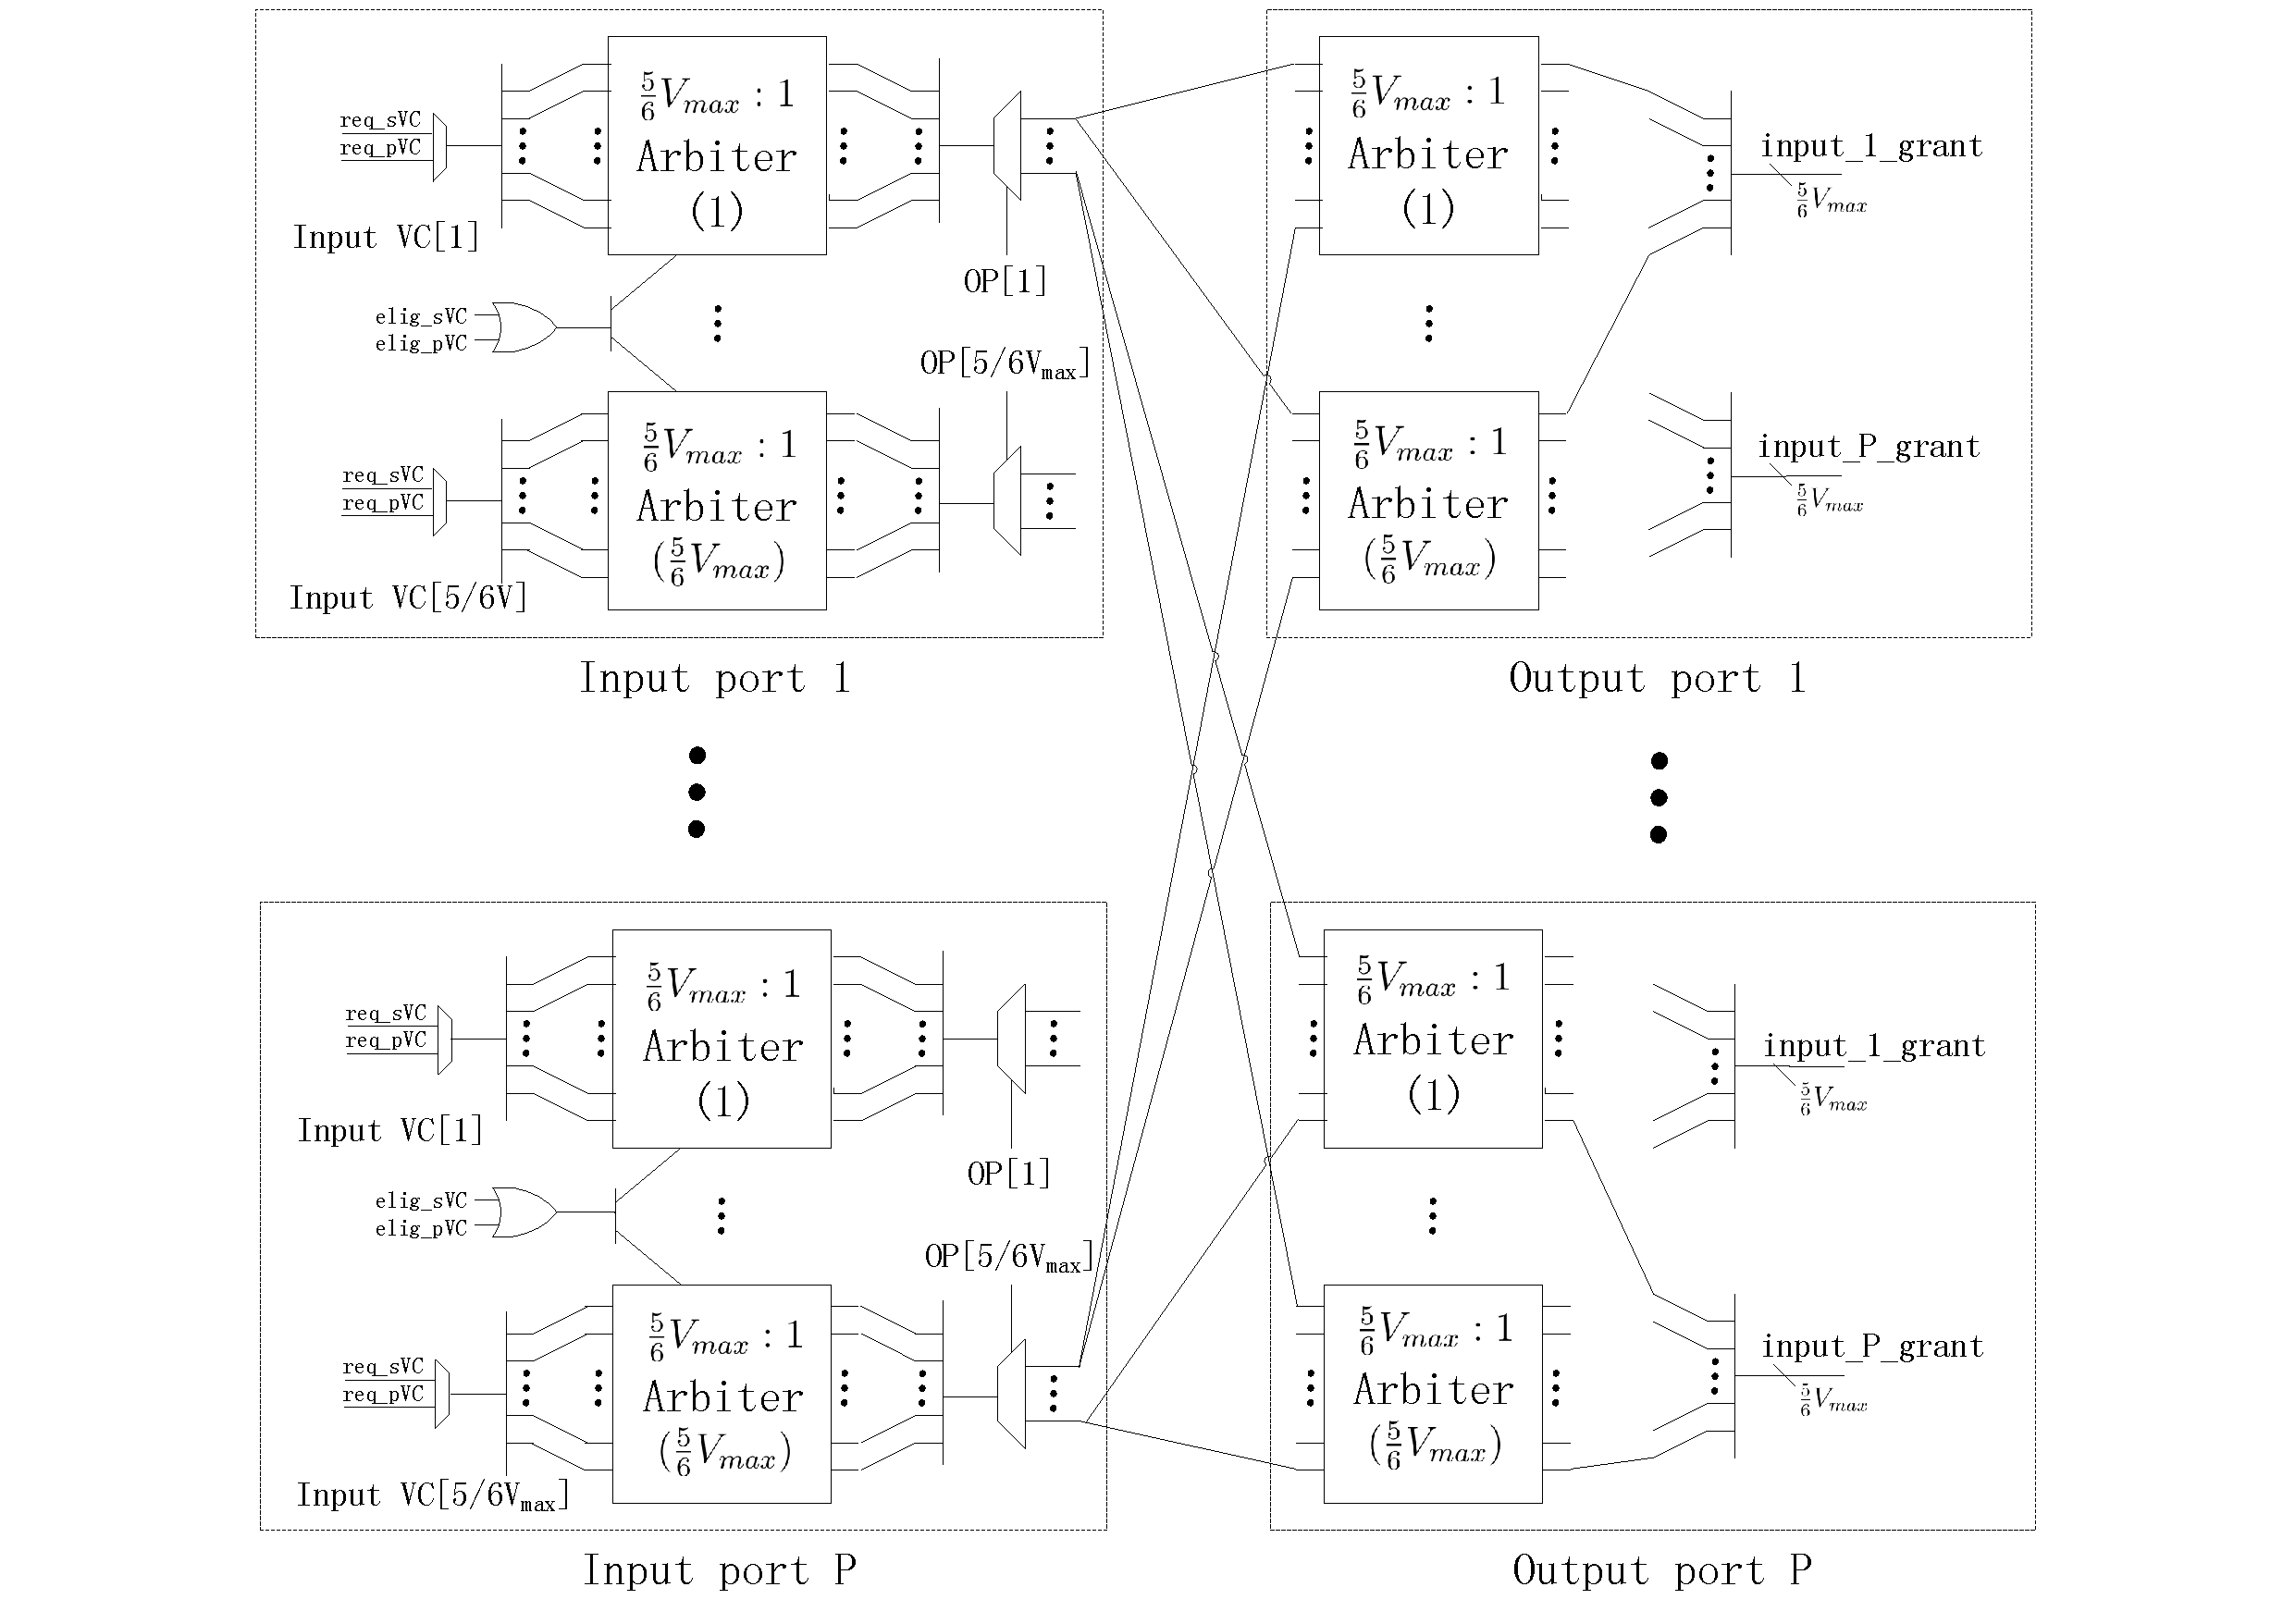
\includegraphics[scale=0.25]{figures/vcalloc.pdf}
\caption{The Implementation of VCA}\label{vcallocator}
\end{figure}

Similarly, for the SWA, if one of the VC is blocked due to some reasons, the corresponding request port can be reused by the shared VC. As shown in Fig. \ref{swallocator}, we first use a $2:1$ arbiter to select on request from either shared VC or private VC at the first stage. The selection is performed in round-robin order to avoid livelock. The second stage utilizes a $1/2V_{max}:1$ arbiter at each input port to select one winner from all the request. Then, a third stage with a $P:1$ arbiter at each output port is applied to select one request for each output. In contrast, to meet the same arbitration demand, the separable input-first allocator used in typical router needs $V_{max}$ $V_{max}:1$ arbiters to guarantee at most 1 input VC be granted, and each output port employs a $P:1$ arbiters to grant to a unique input VC. We will demonstrate the hardware saving of our proposal in subsection \ref{area}.
\begin{comment}
我们的交换机分配器为$P\times V_{max}$个请求分配$P$个输出端口资源,如图\ref{swallocator}。与虚通道仲裁器类似,由于影子vc和私有vc 共享同一个sw/va请求端口,因此我们需要在该端口上增加一个$2:1$ 的优先级分配器来选择一个请求输入到分配器中.为了让共享虚通道尽快排空队列以适应流量的变化,我们给影子vc 赋预较高的优先级。接下来我们为每个输入端口设置1个$5V_{max}/6:1$的仲裁器用于从该端口中选择一个vc 作为下一时钟的备选输出vc;并为每个输出端口设置1个$P:1$ 的仲裁器用于选择一个输入端口。在进行交换机分配时需要考虑下游路由器的可用缓存大小,因此信约值会做为交换机分配的依据。我们的方案在第二阶段与经典的路由器结构相同,但是在输入阶段采用的仲裁器规模更小。对于仲裁器的面积和功耗我们将在\ref{experiemnts} 节进行详细的比较。
\end{comment}
\begin{figure}
\centering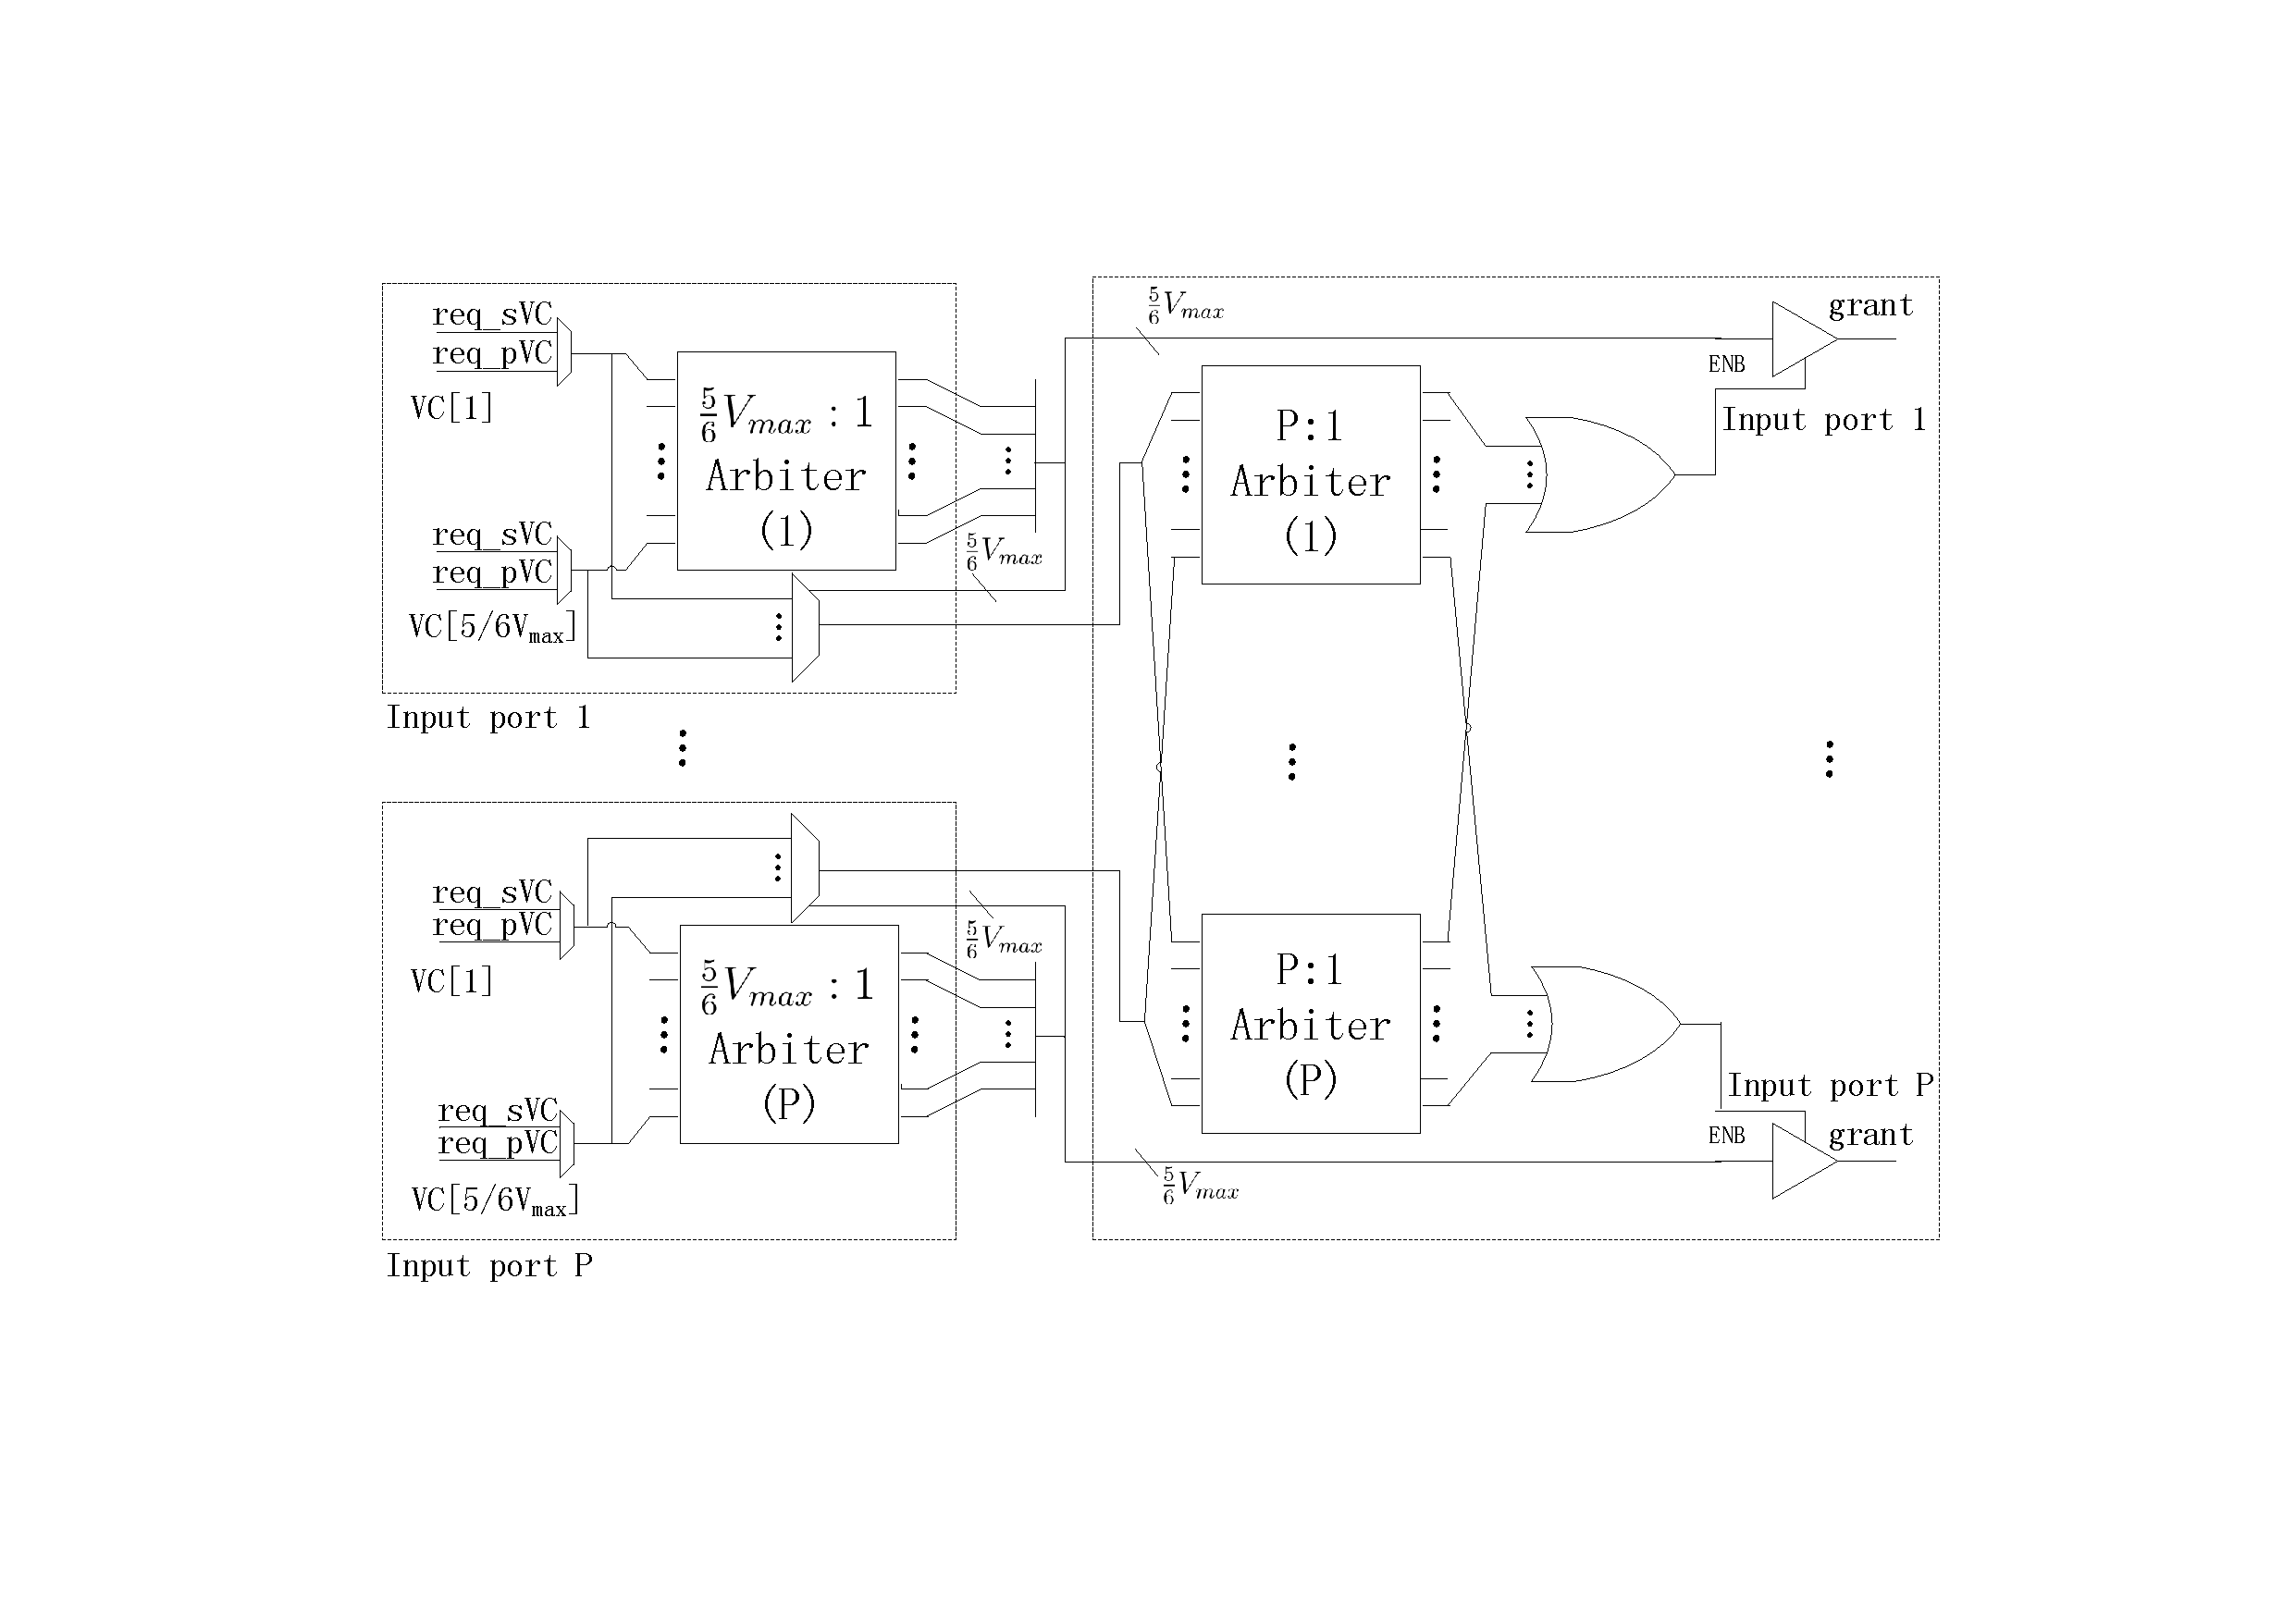
\includegraphics[scale=0.3]{figures/swalloc.pdf}
\caption{The Implementation of SWA}\label{swallocator}
\end{figure}

\section{Experimental results}\label{experiemnts}
To compare the performance and hardware overhead of our approach with existing proposals, we implement AVCS router, typical router \cite{DaTo01} and dynamical buffer management router \cite{NPKV06}\cite{4555894} in Verilog HDL. The comparison results on hardware overhead, network performance, power and chip area are presented in the following three subsections.
\begin{comment}
为了评价our approach的优劣,我们基于Verilog HDL设计并实现了我们的路由器方案Cononical以及经典路由器结构和基于链表组织的动态缓存管理方案LL。 baseline 路由器同样采用基于链表的动态缓存管理方案,基于虫孔交换的标准5段流水线的片上网络,采用基于信约的流量控制,路由算法采用维序路由,拓扑结构为Mesh结构,因此每个路由器有5个端口。每个缓存器的容量为x个切片,每个切片为64bit 宽。每个端口共有10 个私有vc,共享缓存共有10个影子vc。在接下来的三个小节中,我们分别比较和评估我们的方案与Cononical和LL两种基准路由器在需要的硬件控制逻辑、性能、功耗、面积等方面的优势。
\end{comment}

\subsection{Control Overhead Comparison}\label{controllogic}
Both UBS \cite{NPKV06}\cite{5770788} and LLB \cite{4555894}\cite{Neishaburi:2009:RAN:1531542.1531658} require large amount of control logic to keep track of buffer usage. For the inter-port buffer sharing scheme \cite{Neishaburi:2009:RAN:1531542.1531658}, the hardware overhead is much higher than the intra-port sharing scheme since the Next Pointer and Free Slot Pointer for each input port, the Header Pointer and Tail Pointer for each VC must be able to index all the buffer slot within a router. Supposing dynamical buffer management router \cite{NPKV06}\cite{4555894}\cite{Neishaburi:2009:RAN:1531542.1531658}\cite{5770788} has $B$ buffer slots and $V$ VCs at each input port. Then, our approach has $5/6V$ private VCs and $5/6B$ buffer slots at each input port, and each shared buffer bank has $1/6B$ buffer slots and $1/6V$ shared VCs. For each input port of UBS router, denote by $L$ the packet length. Under the same condition, the VC Availability Tracker and Slots Availability Tracker require $V+\lceil log_2 V\rceil$ and $B+\lceil log_2B\rceil$ registers, respectively; The VC Control Table needs $VL\lceil log_2B\rceil$ registers; Both the Arriving and Departing Flit Pointers require $2V\lceil log_2 L\rceil$ registers. For each input port of LLB router, the Free Slots Table requires $B$ registers to track the unused slots and $\lceil \log_2 B\rceil$ registers to point to the first available slot; The Next Pointers Table requires $B\times \lceil log_2 B\rceil$ registers to maintain the flits order of all the VCs; Both the Head Pointers Table and Tail Pointers Table need $V\times \lceil log_2 B\rceil$ registers. Similarly, the hardware overhead of AVCS can be derived, as shown in Table \ref{control}.
\begin{comment}
无论是基于UBC\cite{NPKV06}\cite{5770788}的动态缓存管理结构还是基于链表\cite{4555894}\cite{Neishaburi:2009:RAN:1531542.1531658} 的动态缓存管理,都需要除了缓存器以外的大量的控制存储逻辑来对缓存区进行动态的管理。特别是MH提出的端口间缓存共享的方案\cite{5770788}\cite{Neishaburi:2009:RAN:1531542.1531658} 所需要的控制逻辑更多,因为它要求每个端口的next buffer slot ,header ptr 和tail ptr 应该都是可以寻址到该路由器中任何一个buffer slot的。而在我们的路由器结构中,路由器的缓存被分成了苦干个独立寻址的小块。在同样的缓存容量前提下,我们的路由器结构由于每个memory bank所寻址的地址空间变小,因而所需要的存储控制逻辑(即用来存储next buffer slot ,header ptr 和tail ptr 的寄存器的数量)也相应的减少。
\end{comment}
\begin{comment}
假设每个端口有容量为B的缓存资源,对于之前的方案\cite{NPKV06}\cite{5770788}\cite{4555894}\cite{Neishaburi:2009:RAN:1531542.1531658} 每个端口有$V_{max}$个虚通道,报文长度为$L$;那么在同等条件下,我们的方案中每个端口有$5/6V_{max}$个私有VC 和$5/6B$的私有存储空间,每个共享存储块中含有$1/6B$的存储空间和$1/6V_{max}$个VC. 对于UBC 方案,每个端口的VC Tracker 需要$V_{max}$ 个寄存器,Free Slot Tracker 需要$B$ 个寄存器,VC Control Table 需要$V_{max}Llog_2B$ 个寄存器;对于一个5 个端口的路由器所需要的总的控制开销为$V_{max}+B+V_{max}Llog_2B$。 对于Lai 提出的基于链表的端口内缓存共享方案\cite{4555894},每个端口的free buffer tracker的开销为$B\times log_2 B$,header pointer的开销是$V_{max}\times log_2 B$,tail pointer 的开销是$V_{max}\times log_2 B$,下一跳指针的开销$B\times log_2 B$;5个端口总的控制开销为$10\times(B+V_{max})\times log_2B$。采用同样的方法可以推导出MH提出的两种端口间缓存共享方案\cite{5770788}\cite{Neishaburi:2009:RAN:1531542.1531658} 以及我们的方案的控制存储开销,如表\ref{control}所示。
\end{comment}
\begin{table}
\caption{Hardware overhead comparison}\label{control}
\centering\begin{tabular}{c|c}
\hline
\hline
Structure & Control Register\\
\hline
UBS \cite{NPKV06}  &   $5((V+B)+(1+LV)\lceil log_2B\rceil+\lceil log_2V\rceil+2V\lceil log_2L\rceil)$\\
\hline
LLB \cite{4555894} & $5(B+(1+B+2V) \lceil log_2B\rceil)$\\
\hline
AVCS    & $5(B+(1+\frac{5}{6}B+\frac{10}{6}V)\lceil log_2\frac{5}{6}B\rceil +(1+\frac{B}{6}+\frac{2}{6}V)\lceil log_2\frac{B}{6}\rceil)$\\
\hline
\end{tabular}
\end{table}

To make concrete comparison, for the same packet length $L=8$ flits, we plot the hardware overhead of each scheme under different VC number and buffer capacity in Fig. \ref{bufcmp1} and Fig. \ref{bufcmp2}. As shown in these two figures, our approach uses the lest control logic, because we divide the buffer resources into several banks, and each bank manages their own buffer resource independently. The total hardware overhead is greatly reduced since the addressing space of each buffer bank is smaller than the other two approaches. When the flit width, VC number, buffer size, packet length are 128bits, 12, 24 flits, 8 flits, respectively, the total hardware overhead of our approach is only 5.37\%, in contrast with 7.16\% and 16.24\% of LLB and UBS approach, respectively. We also need to emphasize that although our proposal introduces additional hardware overhead, the utilization improvement makes it possible to halve the buffer slots without degrading the performance, as presented in the following subsection. Thus, our proposal is cost-efficient.
\begin{comment}
为了比较这几种方案所需要的缓存资源,我们假设三种方案使用同样的缓存容量的情况下,对不同的参数值,我们将所需要的控制资源数量画在图\ref{comparions} 中。从图中可以看出,在所有三类参考设计中,在我们的方案是消耗硬件最少的一种。在VC数量为x,缓存容量为X,切片宽度为X时,我们的方案引入的控制存储开销仅为X。我们还需要说明的是,虽然采用共享存储的方式增加了控制逻辑的复杂度,但是提高了性能和缓存利用率。以VichaR为例,实现同样的性能只需要传统路由器50\%的存储资源。端口间的缓存共享可以提高buffer的利用率,使得采用较少的buffer 实现较高的性能成为可能。但是,MH提出的方案完全的端口间缓存共享\cite{5770788}\cite{Neishaburi:2009:RAN:1531542.1531658} 需要非常复杂的逻辑支持以及大量的硬件支持,而这些复杂的硬件又会进一步增加系统的功耗。我们的方案实际上是在不共享和完全共享之间的一个折衷,通过仅共享一部分缓存空间,我们使用对共享缓存的控制存储开销大大降低。
\end{comment}
\begin{figure}
  \centering
  \subfloat[30 buffer slots per port]{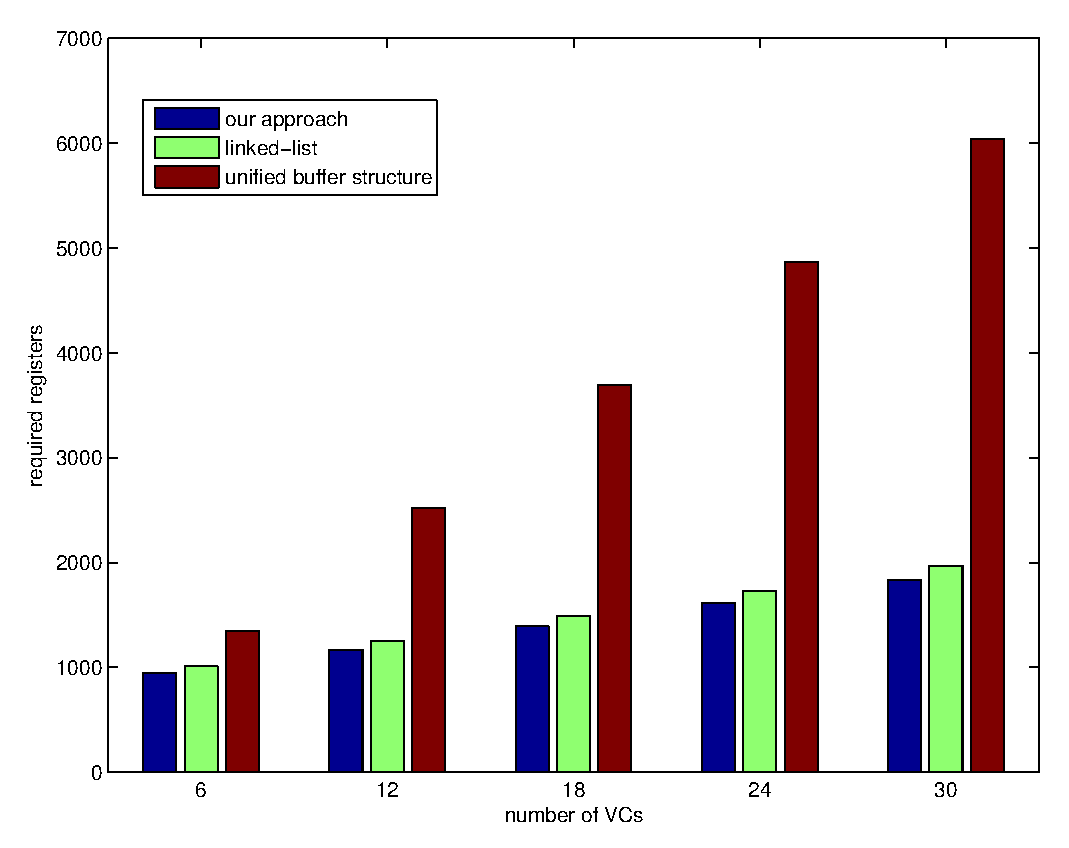
\includegraphics[scale=0.23]{figures/bufcmp1.eps}\label{bufcmp1}}\hspace{10pt}
  \subfloat[12 VCs per port]{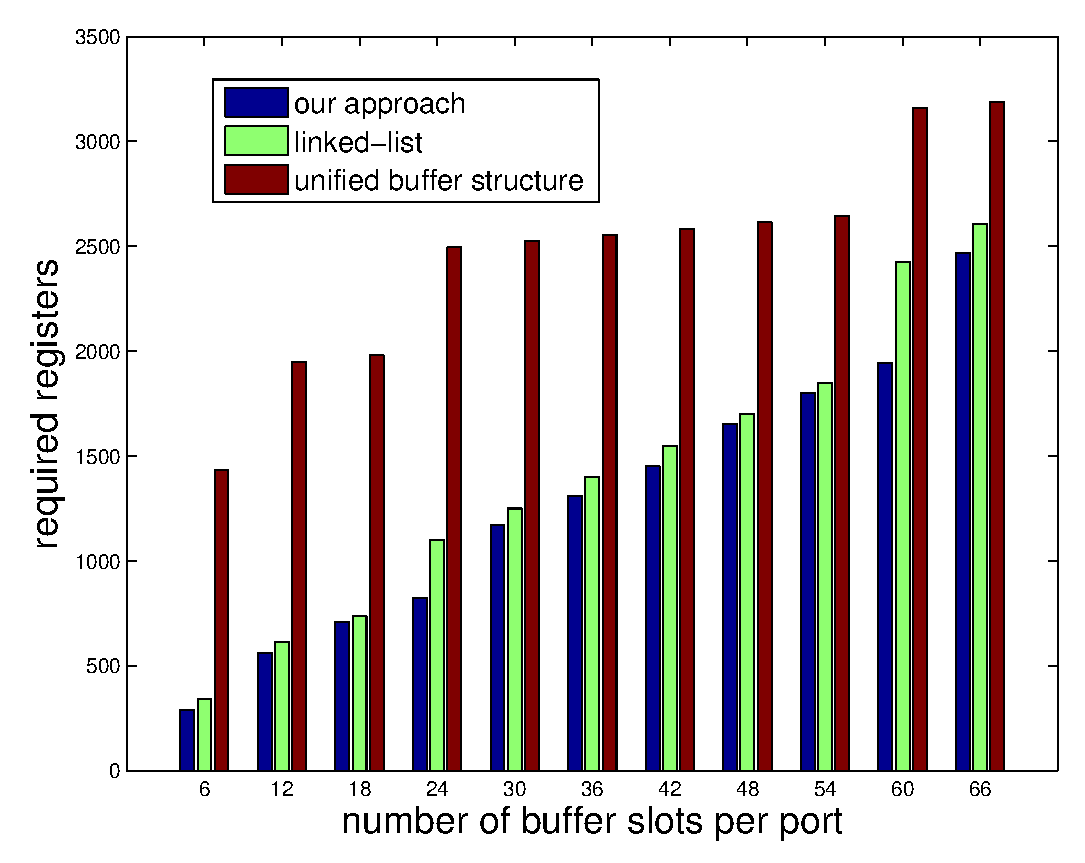
\includegraphics[scale=0.23]{figures/bufcmp2.eps}\label{bufcmp2}}
  \caption{Hardware Overhead Comparison}\label{bufcmp}
\end{figure}

\subsection{Performance Comparison}
In this subsection, we compare the performance of our AVCS router with typical router \cite{DaTo01} and dynamical buffer management router \cite{NPKV06}\cite{4555894} under synthesis traffic pattern and realistic traffic pattern.
\subsubsection{Synthesis Traffic}
Hotspot and uniform traffic pattern are taken as examples to demonstrate the performance improvement of our proposal over the other two kinds of architectures. The configuration used in our experiment are presented in Table \ref{config}. For typical router architecture, two configurations, i.e. Gen(8,24) and Gen(8,48), are used in our comparison according to their VC number and buffer capacity. The dynamical buffer management router architecture is deployed with 12 VCs and 24 buffer slots per input port, denoted as DBM(12,24). To make a fair comparison, we let each input port of our AVCS router have 20 buffer slots and 10 VCs. The shared buffer have 20 buffer slots and 10 VCs in total, organized as five banks. In this experiment, we set the threshold $K=10$.
\begin{comment}
为了比较我们的方案与现有经典路由器结构和基于链表的动态缓存管理方案的性能优劣,我们假设网络拓扑结构为4x4的mesh,报文长度为8个切片。对于典型的基于链表的路由器结构,我们假设每个端口有12个虚通道,24个切片的缓存容量。对于我们的结构,为了保证与经典结构有相同的配置,我们假设每个端口有10个私有虚通道和20 个切片的缓存容量,共享缓存容量为20个切片,虚通道共有10个。我们假设packet source 的缓冲区无限大,暂时无法进入网络的报文将被缓存中源端。我们以均匀流量以及热点流量(热点为0号结点)为例来比较我们的方案与经典路由器和基于链表的路由器结构。设置预热周期为$10^4$ 拍,测量周期为$10^5$ 拍,所得的实验结果如图\ref{lat} 所示.
\end{comment}
\begin{table}[htbp]
\centering
\caption{\label{arcpara}Configuration used in the experiments}\label{config}
\begin{tabular}{|c|c||c|c|}
\hline
network topology    & $4\times 4$ mesh  &   routing algorithm & DOR\\
\hline
flit width   & 256 bits & warmup period &   $1\times 10^4$ cycles\\
\hline
packet length & 8 flits & sampling period &   $1\times 10^6$ cycles\\
\hline
\end{tabular}
\end{table}

As shown in Fig. \ref{hotspotlat}, we find that our approach improves the performance of typical router and dynamical buffer management router under hotspot traffic significantly, take the injection rate 0.00656 flits/node/cycle as an example, our router reduces the average latency over DBM(12,24), Gen(8,24) and Gen(8,48) by 30.1\%, 61.3\% and 29.6\%, respectively. For the uniform traffic, our approach achieves the similar performance as DBM(12,24) and Gen(8,48), but improves the performance of Gen(8,24) significantly, as shown in Fig. \ref{randomlat}. Our inter-port VC sharing router does not achieve too much gain while comparing with dynamical buffer management router because the congestion status of each input port under uniform traffic pattern is similar.
\begin{comment}
通过实验,我们发现,我们的方案在热点流量情况下性能改进非常很明显,以注入速率0.005为例,我们的路由器性能提升15\%. 而热点流量恰是Cache 一致性能及MC访问的重要应用场景。从图中还可以看出,我们的方法对于均匀流量来说造成了一定的性能下降,原因是对于均匀流量来说,每个路由器端口的拥塞程序通常很接近,因而端口间缓存共享带来的性能提升非常有限。而在热点流量情况下,端口间的流量分布是严格不均匀的,因而我们的方案可能会得到更大的收益。此外,我们还比较了两种路由器结构在transpose流量模式下在饱和点附近的平均延迟情况,结果显示我们的方案在K=x时性能提升x\%.
\end{comment}
\begin{figure*}
  \centering
  \subfloat[hotspot traffic pattern]{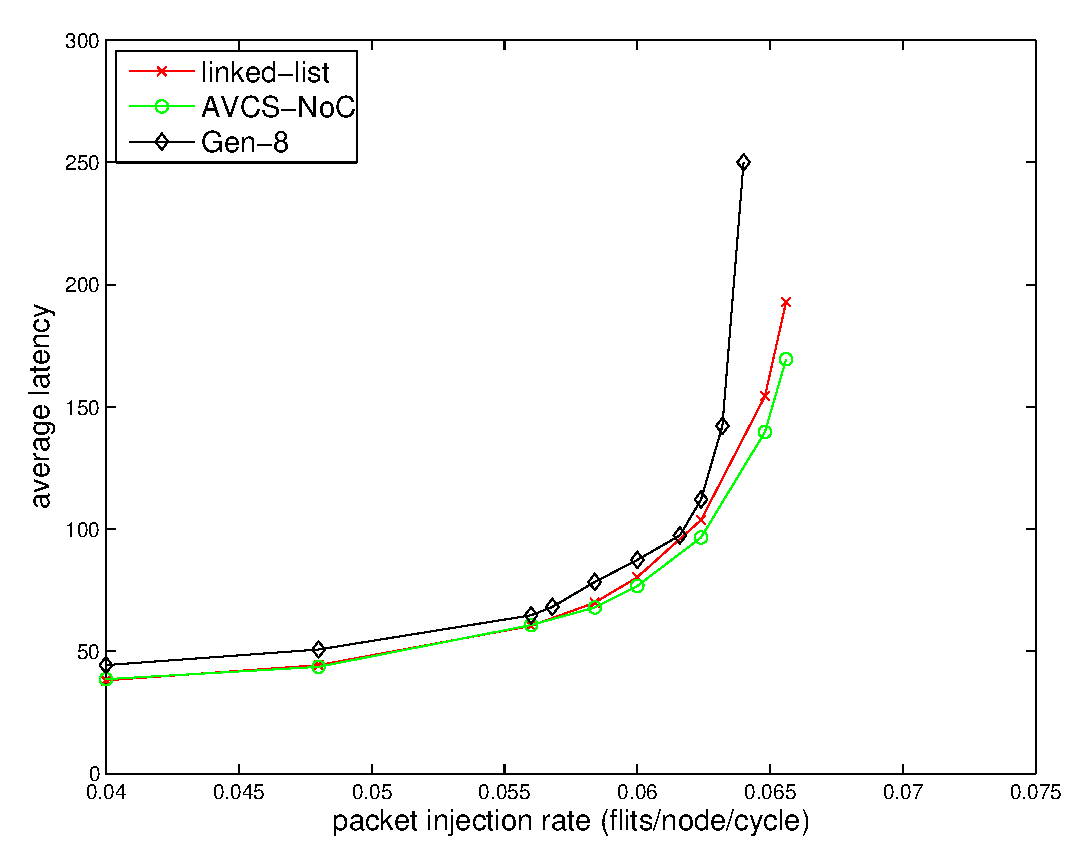
\includegraphics[scale=0.3]{figures/hotspotlat.eps}\label{hotspotlat}}\hspace{10pt}
  \subfloat[uniform traffic pattern]{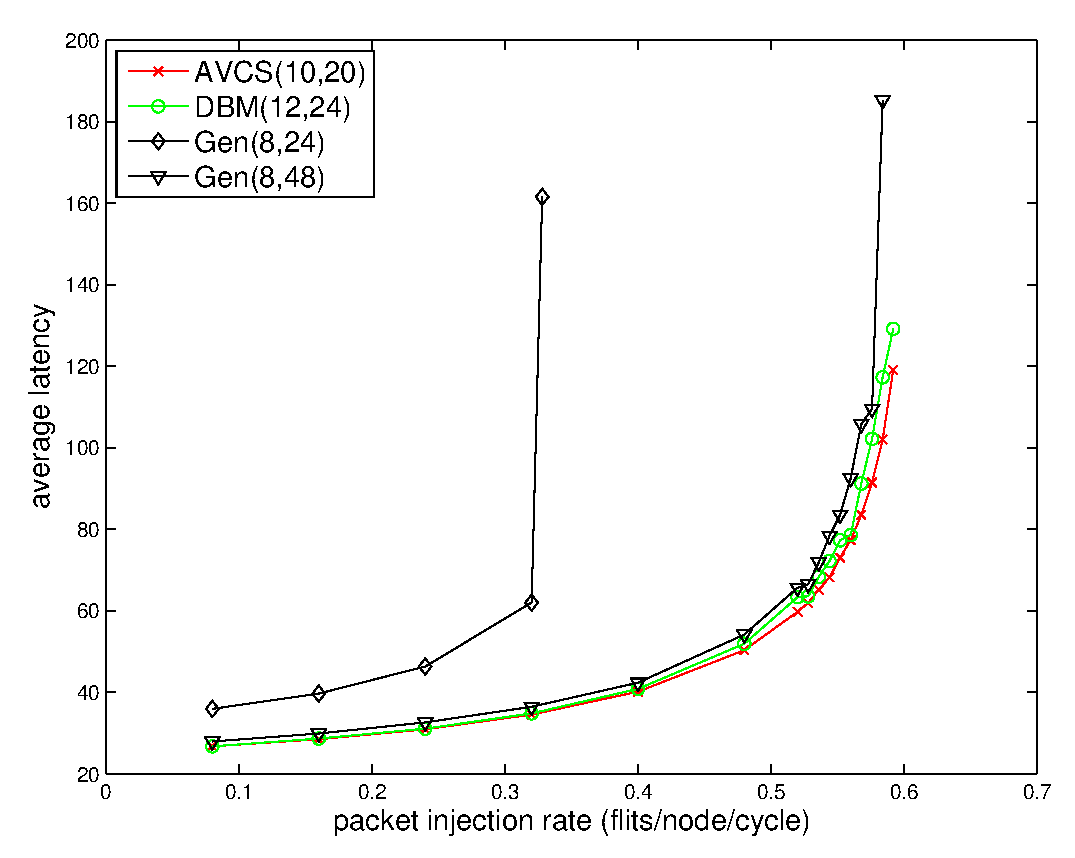
\includegraphics[scale=0.3]{figures/randomlat.eps}\label{randomlat}}\hspace{10pt}
  \subfloat[transpose traffic pattern]{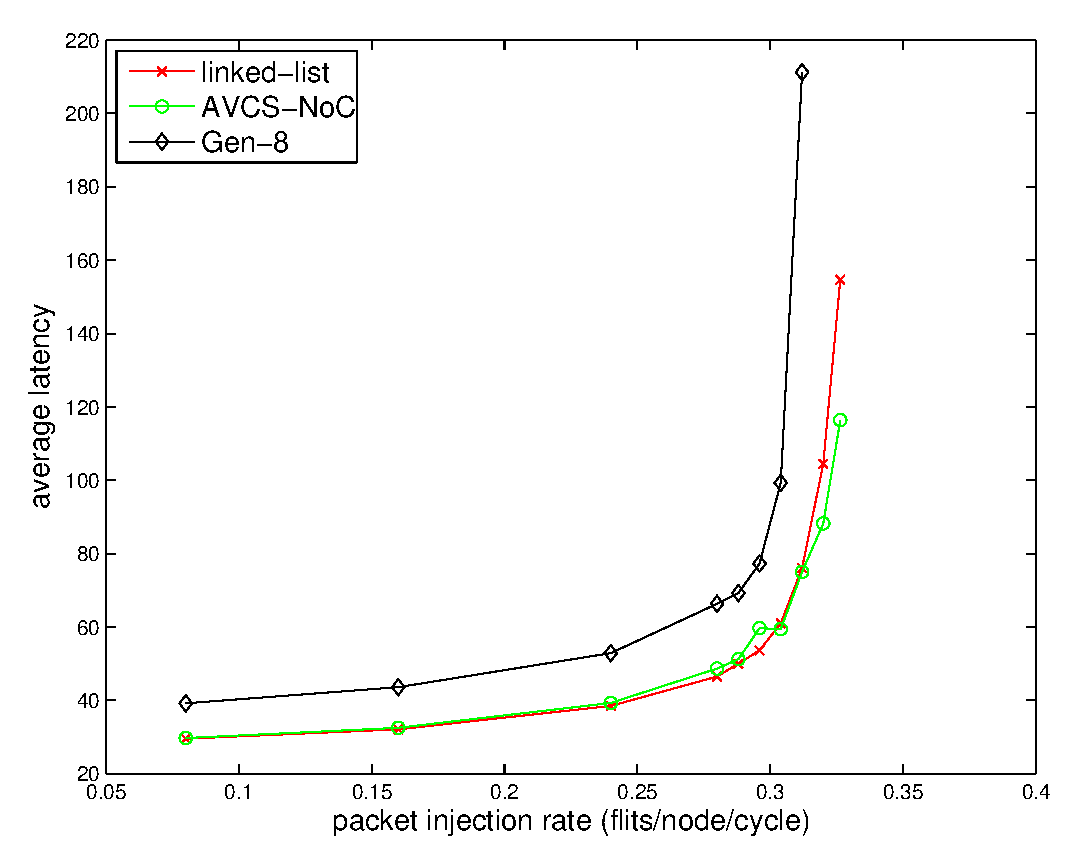
\includegraphics[scale=0.3]{figures/transposelat.eps}\label{transposelat}}
  \caption{Latency comparison}\label{lat}
\end{figure*}

\subsubsection{Realistic Traffic}
For the realistic applications, the workload of each router port is different and changes with time. Our proposal can adapt this dynamical change and allocate more buffer and VC resources to meet the resource requirement of input ports with higher traffic load. This property makes our approach more promising than the other two router architectures. We take two real-world applications, i.e. Video Object Plan Decoder (VOPD) \cite{6553191} and Multi-Window Display (MWD) \cite{1374853}, as examples to compare the performance of our proposal with Gen(8,24), Gen(8,48) and DBM(12,24). These two applications are mapped to $4\times 4$ and $4\times 3$ mesh NoC, as shown in Fig. \ref{vopd} and Fig. \ref{mwd}. The communication rate (flits/cycle) is labelled on the channel connecting two routers.
\begin{comment}
在实际的应用中,端口之间的流量分布通常是不均匀的,因此我们的方案较之前的方案会有较大的性能提升。我们以Video Object Plan Decoder (VOPD)应用\cite{Tol2001}来验证这一点。该应用共有16个子任务组成,将其采用NMAP映射算法\cite{1269002}映射到$4\times 4$的Mesh网络后如图\ref{vopd}所示,每个链路上的数字表示两个任务之间的通信速率(in flits/cycle)。我们分别采用经典路由器结构、基于链表的路由器结构和我们的路由器结构来进行实验,对于同样的路由器缓存容量和虚通道数量(120切片,30 vc in total),我们发现,经典路由器结构中,延迟比另两种路由器结构大1个数量级,而我们的路由器结构较基于链表的路由器结构性能改进9\%。此外,我们还发现当经典路由器结构采用2倍于AVCS路由器的缓存容量时二者的性能相当。这也进一步说明,我们的方案通过实现动态缓存管理和端口间缓存和虚通道共享在很大程度上降低了硬件成本。我们知道,在切片位宽为128bit 时,我们的动态缓存管理结构引入的控制开销为x\%bit,而在采用了动态缓存管理后可以节省的缓存容量为50\%。因此,我们总的存储成本大大下降。
\end{comment}
\begin{figure*}
  \centering
  \subfloat[Video Object Plan Decoder]{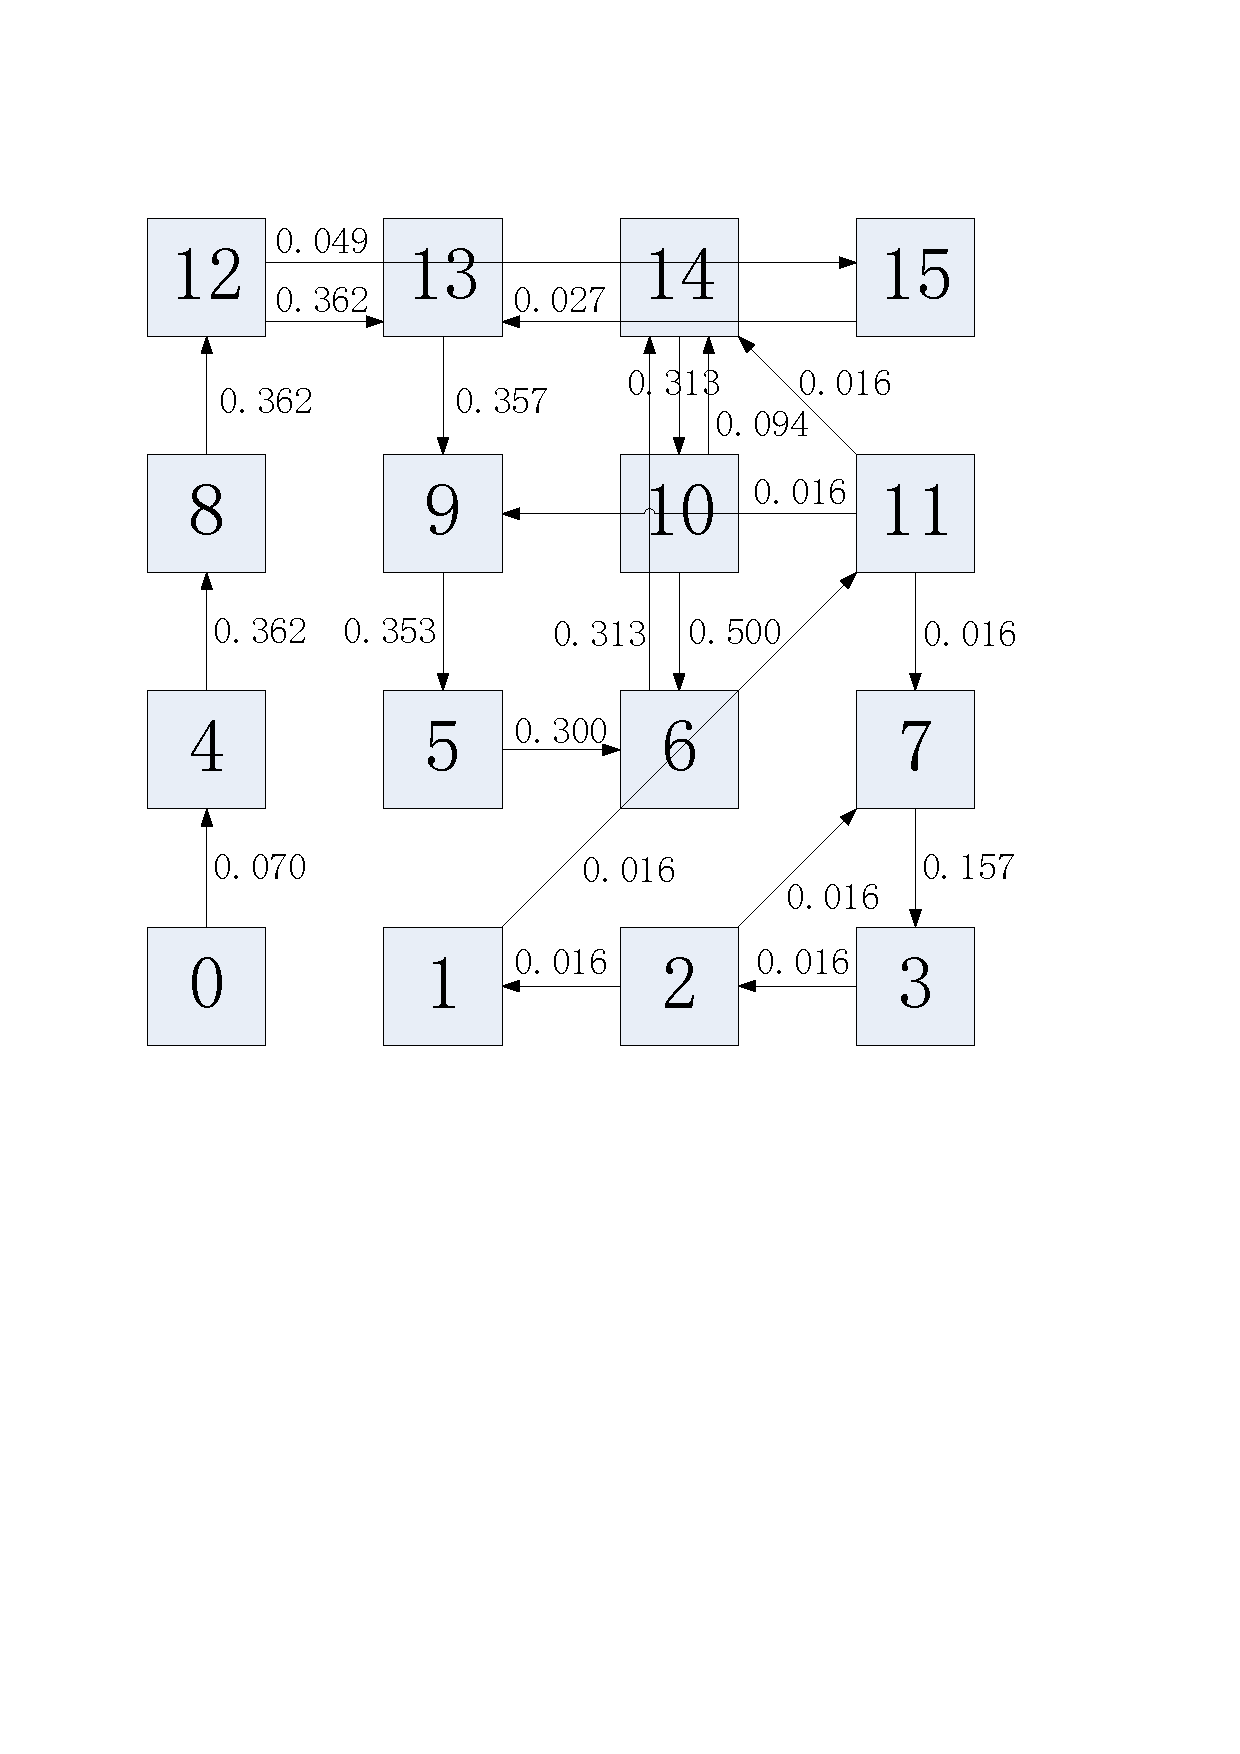
\includegraphics[scale=0.32]{figures/vopd.pdf}\label{vopd}}\hspace{10pt}
  \subfloat[MPEG4 Decoder]{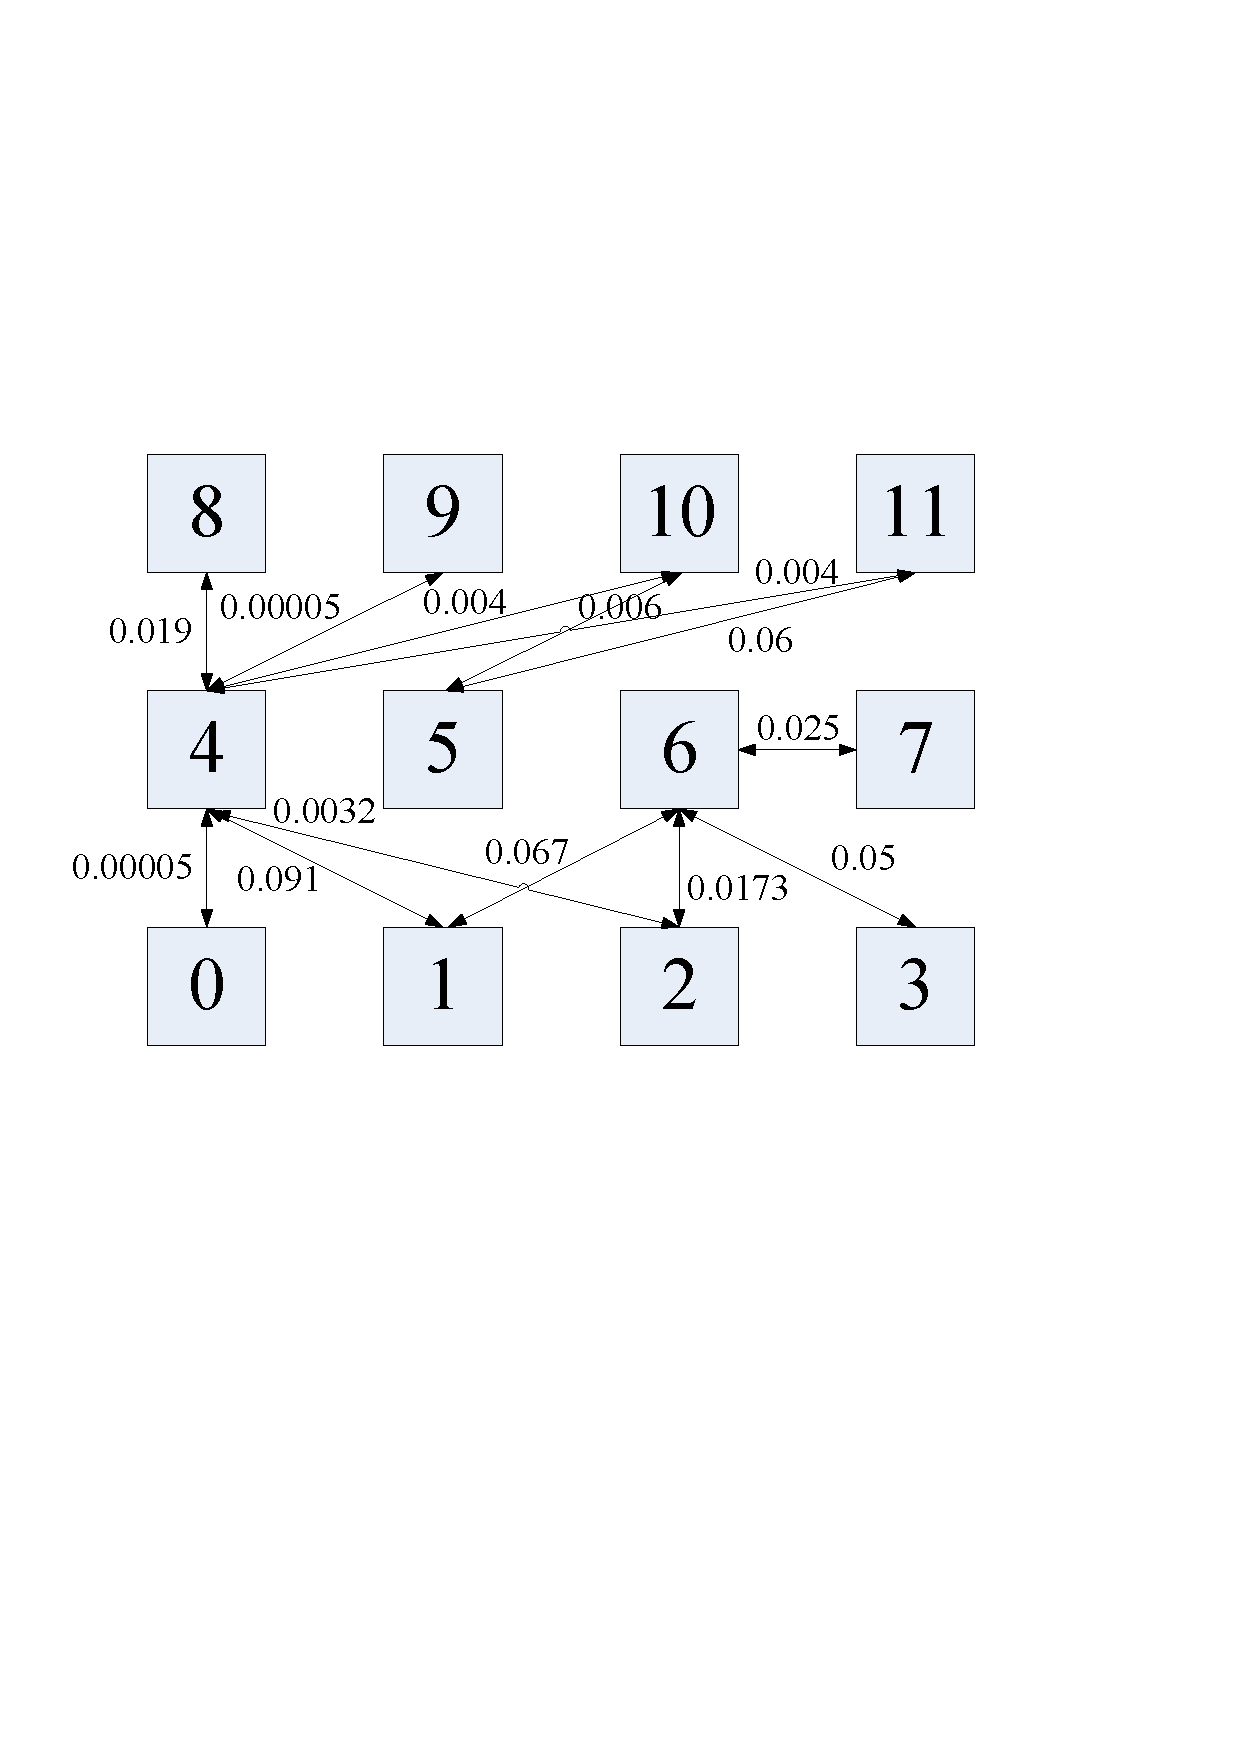
\includegraphics[scale=0.32]{figures/mpeg4.pdf}\label{mpeg4}}\hspace{10pt}
  \subfloat[Multi-Window Display]{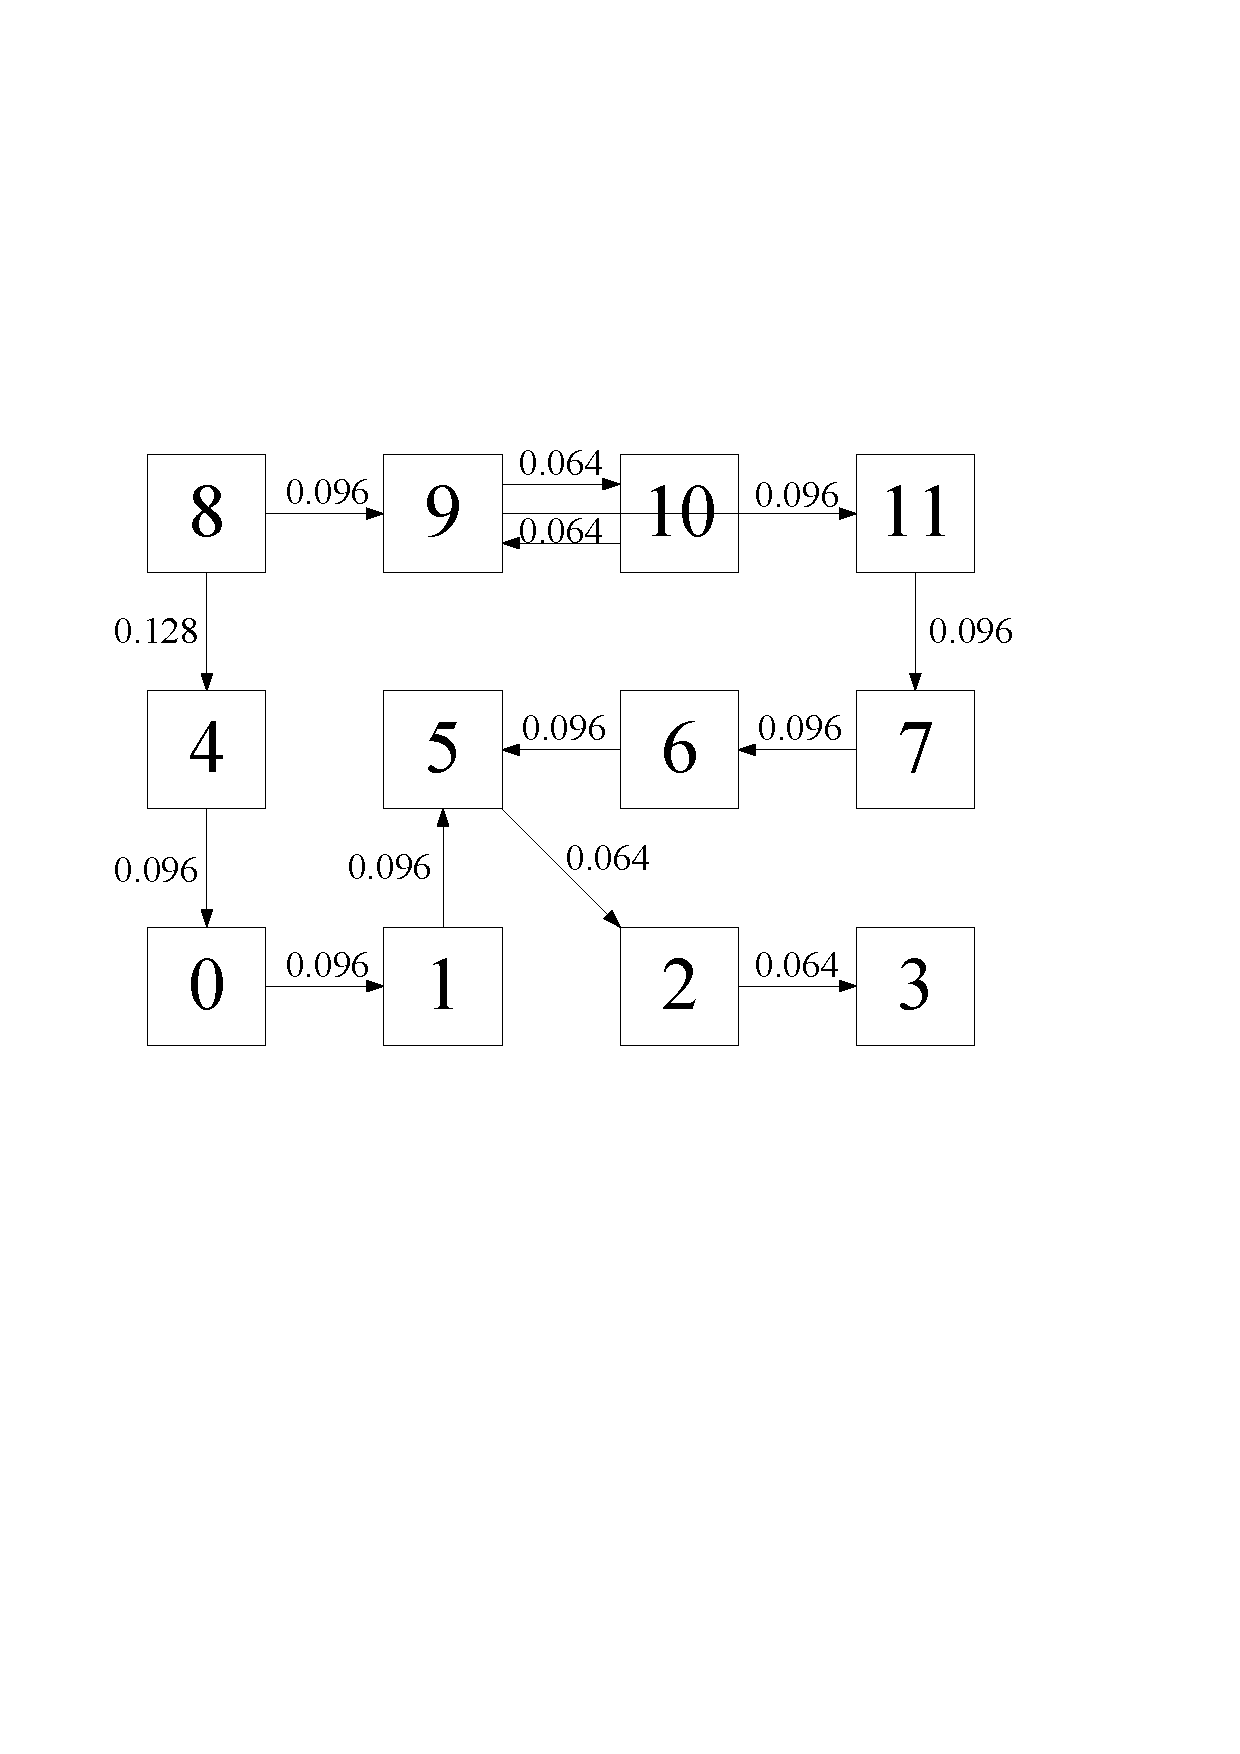
\includegraphics[scale=0.32]{figures/mwd.pdf}\label{mwd}}
  \caption{Task mapping of three applications on mesh topology and corresponding injection rate (flits/cycle)}\label{realistic}
\end{figure*}

\begin{table}
  \centering\caption{Simulation configuration}\label{configure}
  \begin{tabular}{|c|c||c|c|}
    \hline
    Network topology & $4\times 4$ mesh  &   routing algorithm & DOR\\
    \hline
    Packet length & 10 flits & threshold & 1 cycle\\
    \hline
    warmup period &   $1\times 10^4$ cycles & sampling period &   $1\times 10^5$ cycles\\
    \hline
    \end{tabular}
\end{table}

For the given configuration listed in Table \ref{configure}, we run the simulation with the detailed RTL implementation of these three router architectures for all these applications. The experimental are presented in Table \ref{realisticapp}. The experimental results show that, AVCS achieves better performance than LLB(12,24), Gen(8,24) and Gen(8,48). This is because our structure improves the buffer utilization and reduces the blocking caused by VC insufficiency, which makes it possible to achieve better performance by utilizing fewer buffer space.
\begin{table*}
  \centering\caption{Average latency comparison (in cycles)}\label{realisticapp}
\begin{tabular}{|c|c|c|c|c|}
\hline
 & AVCS(10,20) & Gen(8,24) & Gen(8,48) & DBM(12,24)\\
\hline\hline
VOPD & 29.3805 & 606.31 ($\downarrow$ 95.2\%) & 29.9462 ($\downarrow$ 1.9\%) & 29.5593 ($\downarrow$ 0.6\%)\\
\hline
MPEG4 & 25.4454 & 32.0747 ($\downarrow$ 20.7\%) & 25.4935 ($\downarrow$ 0.2\%) & 25.4578 ($\downarrow$ 0.04\%)\\
\hline
MWD & 22.4489 & 30.0246 ($\downarrow$ 25.2\%) & 22.5405 ($\downarrow$ 0.4\%) & 22.4777 ($\downarrow$ 0.1\%)\\
\hline
\end{tabular}
\end{table*}

\subsection{Power and Area Comparison}\label{area}
The detailed RTL implementation of AVCS and typical router are synthesized with Synopsys Design Compiler under FreePDK 45nm standard cell library \cite{nangate}. We configure medium effort optimization option for the synthesis tool and set the working voltage and frequency to 1.1V and 200MHz. For AVCS(10,20) router, the power consumption with assumed switching activity factor 10\% is 141.445 mW, chip area is 1002486.625 $\mu^2 m$. In contrast, Gen(8,48) consumes 208.224 mW power and occupies 1135084.5 $\mu^2 m$ chip area under the same conditions, which saves 11.7\% chip area and reduces 32.1\% power consumption. We compared the power and area overhead of AVCS(10,24) with Gen(8,48) since they achieves the similar performance under both synthesis and realistic traffic patterns.
\begin{comment}
为了展示我们提出的体系结构的性能优势以及成本等特点,我们采用Verilog 实现了一个时钟精确的noc 路由器模型,该模型通过Synopsys 工具进行综合,采用的工艺库是open-source process design kit FreePDK 45nm Standard Cell Library 工艺库\cite{nangate},工作电压设置为1.1V。 在主频200MHz 时:对于动态分配的片上网络路由器结构,动态功耗为99.4796mW,芯片面积为827262.788363,而我们的方案功耗为101.8994mW,面积823642.608870. 经过比较发现我们的方案功耗提高2\%,但是占用的芯片面积下降0.4\%.
\end{comment}

Finally, we compared the chip area and power consumption of our revised VCA and SWA with that of used in typical router. Supposing each router has $P$ input ports and each port has $V$ VCs. Then, a $PV\times PV$ VCA and a $PV\times P$ SWA should be deployed in typical router, while our approach uses a $5/6PV\times 5/6PV$ VCA and a $5/6PV\times P$ SWA instead. We let $P=5$ and change V from 6 to 24 with step 6, the power and chip area of these two schemes are listed in Table \ref{alloccost}. As shown in this table, our approach saves more chip area than the typical allocator structure. In addition, our approach tends to save more power consumption than the baseline allocator structure when the more VCs are supported.
\begin{comment}
另外,我们还比较了我们基于影子vc的虚通道和交换机分配模块的芯片面积和功耗。假设基准路由器有5个端口,每个端口的vc数量为$V_{max}$,那么基准路由器中vc分配模块和sw分配模块的规模均为$V_{max}\times V_{max}$,相应的,我们的方案中两个分配器的规模均为$5/6V_{max}\times 5/6V_{max}$。设置工作电压1.1V和工作频率200MHz,我们比较了两种方案的面积和功耗,如表\ref{alloccost}所示。从表中可以看出,我们的方案在面积方面始终都优于之前的方案。随着虚通道数量的增加,我们的方案功耗效率也逐渐超过基准路由器结构。
\end{comment}
\begin{table*}
\centering\caption{Chip area and power consumption comparison with baseline allocator}\label{alloccost}
\begin{tabular}{|c|c|c|c|c|c|c|c|}
\hline
\multirow{2}{*}{$\#$VC} & \multicolumn{3}{|c|}{Area($\mu m^2$)} & \multicolumn{3}{|c|}{Power(mW)}\\
\cline{2-7}
& Baseline & AVCS & AVCS vs. Baseline & Baseline & AVCS & AVCS vs. Baseline\\
\hline
6 & 62013.8828 & 58659.8906 & $\downarrow$ 5.4\% & 5.846 & 6.292 & $\uparrow$ 7.6\%\\
\hline
12 & 221112.5312 & 206178.4062 & $\downarrow$ 6.8\% & 14.916 & 15.276 & $\uparrow$ 2.4\%\\
\hline
18 & 492946.6562 & 426018.5625 & $\downarrow$ 13.6\% & 26.962 & 24.870 & $\downarrow$ 7.8\%\\
\hline
24 & 882065.3750 & 822519.5000 & $\downarrow$ 6.8\% & 38.999 & 38.732 & $\downarrow$ 0.7\%\\
\hline
\end{tabular}
\end{table*}

\section{conclusion and future works}\label{conc}
The buffer organization and management scheme is a key factor which determines the performance of wormhole-switched NoC router. In this paper, we propose a runtime adaptive buffer and VC sharing approach, which dynamically allocates the shared buffer and VCs to the desired input ports to better adapt the traffic condition and improve the network performance. Comparing with existing UBS and LLS approaches, our method introduces the lest hardware overhead and further improve the network performance. Another contribution of this paper is that we proposed the idea of request port sharing, which uses a smaller VCA and SWA to perform the VC and switch allocation. By applying this sharing scheme, the chip area and power overhead of these two components are reduced significantly. The synthesis results show that our approach saves 32.1\% power and 11.7\% chip area while comparing with typical router of the similar performance. For the future work, we plan to realize the fault tolerant and QoS isolation in this architecture.
\begin{comment}
缓存的组织和管理方式是影响基于虚通道的虫孔交换片上网络性能和成本的关键因素。本文中,我们提出一种运行时自适应的缓存和VC分配方案.该方案在网络工作过程中自适应的根据当前流量状态自动的调整缓存和虚通道在各个端口之间的分配,与单纯提高缓存利用率的方法相比,我们的方法可以进一步的提高吞吐率降低平均端到端延迟。本文的另一个贡献是提出了影子VC概念,通过分配器端口复用的方式在不影响怀能的前提下,使得我们可以采用一个较小的VC 和SW分配器来实现对较大规模的分配,进而缩短了路由器中关键路径的长度,进而提高了路由器支持的最高频率。硬件逻辑综合的结果显示,我们的方案与基于链表的方式占用几乎相同的芯片面积和功耗,但是我们的方案在热点流量情况下与经典路由器结构相比改进网络的性能达到x\%,与基于链表的方式相比改进路由器的性能达到x\%。作为将来的工作重点,我们考虑将网络演算理论应用于该体系结构,并考虑在动态vc 分配的基础上实现流量的隔离、服务质量保证和容错。
\end{comment}

\section*{Acknowledgement}
The authors thank the reviewers for their suggestions and comments, and all the experiments are carried out at the Integrated Microsystem Lab (IML) of McGill University. This research is supported by High Technology Research and Development Program of China (Grant No. 2012AA012201, 2012AA011902).

\section*{Conflict of Interests}
The authors declare that there is no conflict of interests regarding the publication of this paper.

\bibliographystyle{unsrt}
\bibliography{Docear}

\end{document}
